\documentclass[8pt, a4paper, fleqn, landscape]{scrartcl}
\usepackage[utf8]{inputenc}
\usepackage[ngerman]{babel}

\usepackage{hyperref}

%Layout
\usepackage{multicol, geometry, xcolor}
\geometry{margin=1cm}
\parindent 0pt
\pagestyle{empty}

\newlength{\breite}
\setlength{\breite}{0.5pt}
\setlength{\columnseprule}{\breite}

\usepackage{graphicx}

\usepackage{tikz}
\usepackage{scalerel} %maybe not needed



%Mathematik-Pakete
\usepackage{amsmath, amstext, amssymb, mathtools, esint, polynom}
\usepackage{bm}
\allowdisplaybreaks %Seitenumbruch in align-Umgebung erlauben


% Farbe der Boxen für Titel / Untertitel
\definecolor{section}{RGB}{79,148,205}
\definecolor{subsection}{RGB}{135,206,250}
\definecolor{titletext}{RGB}{0,0,0}


% section color box
\setkomafont{section}{\mysection}
\newcommand{\mysection}[1]{%
	\Large\sf%
	\setlength{\fboxsep}{0cm}%already boxed
	\colorbox{section}{%
		\begin{minipage}{\linewidth}%
			\vspace*{2pt}%Space before
			\leftskip2pt %Space left
			\rightskip\leftskip %Space right
			{\color{titletext} #1}
			\vspace*{1pt}%Space after
		\end{minipage}%
}}
% subsection color box
\setkomafont{subsection}{\mysubsection}
\newcommand{\mysubsection}[1]{%
	\Large\sf%
	\setlength{\fboxsep}{0cm}%already boxed
	\colorbox{subsection}{%
		\begin{minipage}{\linewidth}%
			\vspace*{2pt}%Space before
			\leftskip2pt %Space left
			\rightskip\leftskip %Space right
			{\color{titletext} #1}
			\vspace*{1pt}%Space after
		\end{minipage}%
}}

				
\providecommand{\diff}{\mathop{} \! \mathrm{d}}


%Informationen für den Befehl maketitle
\title{Physik}
\subtitle{Sammlung, gegliedert nach Modul}
\author{Fabian Suter, \today}
\date{{\small \url{https://github.com/FabianSuter/Physik.git}}}
 
\begin{document}

	\begin{multicols*}{3}
		\maketitle
	 
		\section{Statik}
		
	\subsection{Schwerkraft (Gewichtskraft)}
	
		$$ \boxed{ \text{Allgemein:} \quad F_G = G \cdot \frac{m_1 \cdot m_2}{r^2} }$$
		$$ \boxed{ \text{Erde:} \quad  F_G = G \cdot \frac{m_E \cdot m}{r_E^2} = m \cdot g }$$ 
		
		\begin{tabular}{clc}
			$F_G$ & Gewichtskraft         & $[F_G] = \mathrm{\frac{kg \, m}{s^2} = N}$ \\
			$G$   & Gravitationskonstante & $6.67 \cdot 10^{-11} \mathrm{\frac{m^3}{kg \, s^2}}$ \\ 
			$m_i$ & Massen der Körper     & $[m] = \mathrm{kg}$ \\
			$r$   & Abstand der Massen    & $[r] =\mathrm{m}$ \\
			$g$   & Erdbeschleunigung     & $9.81 \mathrm{\frac{m}{s^2}}$ \\
			$m_E$ & Masse der Erde        & $5.972 \cdot 10^{24} \, \mathrm{kg} $ \\
			$r_E$ & Erdradius             & $6.378 \cdot 10^6 \, \mathrm{m}$ \\
		\end{tabular}
		
	\subsection{Normalkraft (Kontaktkraft)}
		(Sekundär-) Kraft, welche sich so anpasst, dass in Ruhe ein Kräftegleichgewicht herrscht: \\
		\\
		$\boxed{ F_G = -F_N}$ \qquad $\Rightarrow$ im Gleichgewicht auf horizontaler Oberfläche
				
	\subsection{Zerlegung von Kräften}
		Kraftvektoren kann man komponentenweise aufteilen: \\
		\\
		\begin{minipage}{0.6\linewidth}
			\begin{tikzpicture}
				[
				x=1cm, y=1cm, scale=0.7, font=\footnotesize, >=latex 
				%Voreinstellung für Pfeilspitzen
				]
				
				%Raster im Hintergrund
				\draw[step=1, gray, very thin] (0,0) grid (5.5,3.5);
				
				%Länge x Achse
				\draw [-latex] (0,0) -- ++(5.5,0) node[below, scale=1.2] {$x$};
				
				%Länge y Achse
				\draw [-latex] (0,0) -- ++(0,3.5) node[left, scale=1.2] {$y$};
				
				%Winkel
				\filldraw[fill=green!20!white, draw=green!50!black, thick] (1,1) -- (2.5,1) arc (0:26.56:1.5) -- cycle node[midway, below, green!50!black, scale=1.4, yshift=3pt, xshift=5pt] {$\alpha$};		
				
				%Vektor a
				\draw[-latex, very thick] (5,1) -- (5,3) node [midway, right, scale=1.2] {$\vec{F}_y$} node (Fy) {}; 
				%Vektor b
				\draw[-latex, very thick] (1,1) -- (5,1) node [midway, below, scale=1.2] {$\vec{F}_x$} node (Fx) {};

				%\draw[dashed] (a.center) -- ++ (3,0) node (c) {};
				%\draw[dashed] (b.center) -- ++ (2,3);
				\draw[very thick, red, -latex] (1,1) -- (Fy.center) node [midway, above, scale=1.2] {$\vec{F}$} node (F) {};
			\end{tikzpicture}
		\end{minipage}
		\hfill
		\begin{minipage}{0.6\linewidth}
			$\vec{F} = \vec{F}_x + \vec{F}_y + \vec{F}_Z$ \\	
			\\
			\textbf{hilfreich beim Lösen \\
			von Aufgaben!} \\
		\end{minipage}
		
	\subsection{Gleichgewichtsbedingungen für Massepunkte}
		Der Massepunkt erfährt keine Beschleunigung \\
		$\Rightarrow$ Summe aller wirkenden Kräfte ist 0 
		
		$$ \boxed{ \vec{R} = \sum \limits_{i = 1}^n \vec{F}_i = \vec{0} \qquad \Rightarrow \text{komponentenweise} }$$
		
		$$ \boxed{ \sum \limits_{i = 1}^n \vec{F}_x = \vec{0}  \qquad  \sum \limits_{i = 1}^n \vec{F}_y = \vec{0}  \qquad  \sum \limits_{i = 1}^n \vec{F}_z = \vec{0} } $$ 
			
	\subsection{Haftreibung / Gleitreibung}
	
		\subsubsection{Trockene Festkörperreibung}
	
			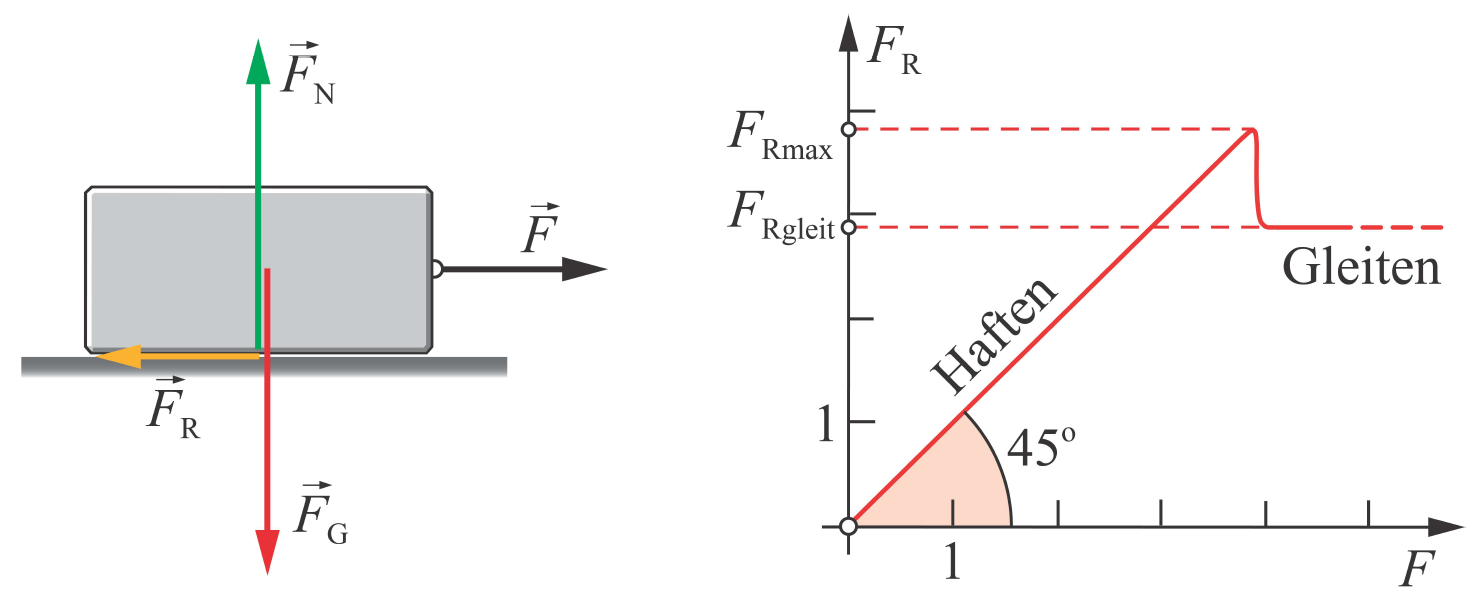
\includegraphics[width=0.7\linewidth]{Bilder/reibung} \\
		
			\begin{minipage}{0.65\linewidth}
				$$ \boxed{ \text{Haftreibung:} \quad \vec{F}_{R,max} = \mu_H \cdot \vec{F}_N } $$ 
				
				$$ \boxed{ \text{Gleitreibung:} \quad \vec{F}_{Gleit} \approx \mu_G \cdot \vec{F}_N } $$
			\end{minipage}
			\hfill
			\begin{minipage}{0.3\linewidth}
				$$ \boxed{ \vert \vec{F}_R \vert \leq \vert \vec{F}_{R,max} \vert } $$ \\
			\end{minipage}
		
			\begin{tabular}{lll}
				$\vec{F}_R$ & Reibungskraft & $[\vec{F}_R] = \mathrm{N}$ \\
				$\vec{F}_{R,max}$ & Haftreibungskraft & $[\vec{F}_{R,max}] = \mathrm{N}$ \\
				$\vec{F}_{Gleit}$ & Gleitreibungskraft & $[\vec{F}_{Gleit}] = \mathrm{N}$ \\
			\end{tabular}

		\subsubsection{Viskose Reibung}
			Sobald Schmiermittel zum Einsatz kommen, ist die Reibungskraft abhängig von der Grösse der Berührungsfläche: \\
			\\
			Bei gleicher Normalkraft $\vec{F}_N$ ist bei 
			
			\begin{tabular}{ll}
				$\bullet$ & kleinerem Flächendruck die Reibung kleiner \\
				$\bullet$ & grösserem Flächendruck die Reibung grösser \\
			\end{tabular}
		
	\subsection{Starre Körper}
	
		\begin{tabular}{ll}
			$\bullet$ & Ein starrer Körper wird durch angreifende Kräfte \\
			& nicht deformiert \\
			$\bullet$ & Bei einem starren Körper kann die Kraft entlang ihrer  \\
			& Wirkungslinie \underline{beliebig} verschoben werden \\
		\end{tabular}
	
	\subsection{Addition von Kräften}
		
		\subsubsection{Spezialfall: Ebene Kräftegruppe für schiefe Wirkungslinie}
			Kräfte entlang ihrer Wikungslinie verschieben \\
			$\Rightarrow$ Im Schnittpunkt vektorielle Addition der Kräfte durchführen, um die resultierende Kraft zu erhalten. \\
			\\
			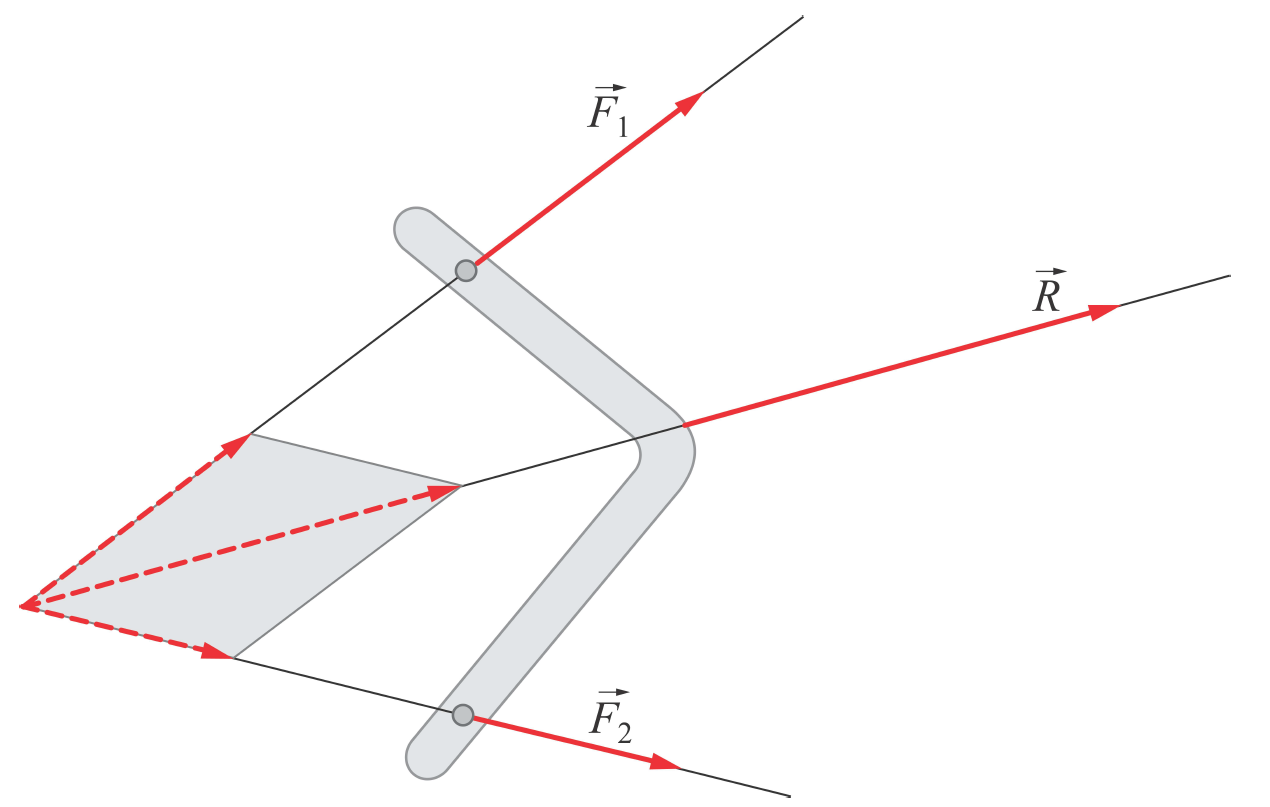
\includegraphics[width=0.7\linewidth]{Bilder/schneidende_wirkungslinien} \\
			\\
			Dieses Verfahren kann auch mehrfach angewendet werden!

		\subsubsection{Spezialfall: Ebene Kräftegruppe für parallele Wirkungslinie}
			Zwei sich zu null addierende Hilfskräfte hinzufügen ($\vec{H}_1 \; , \; \vec{H}_2$) \\
			\\	
			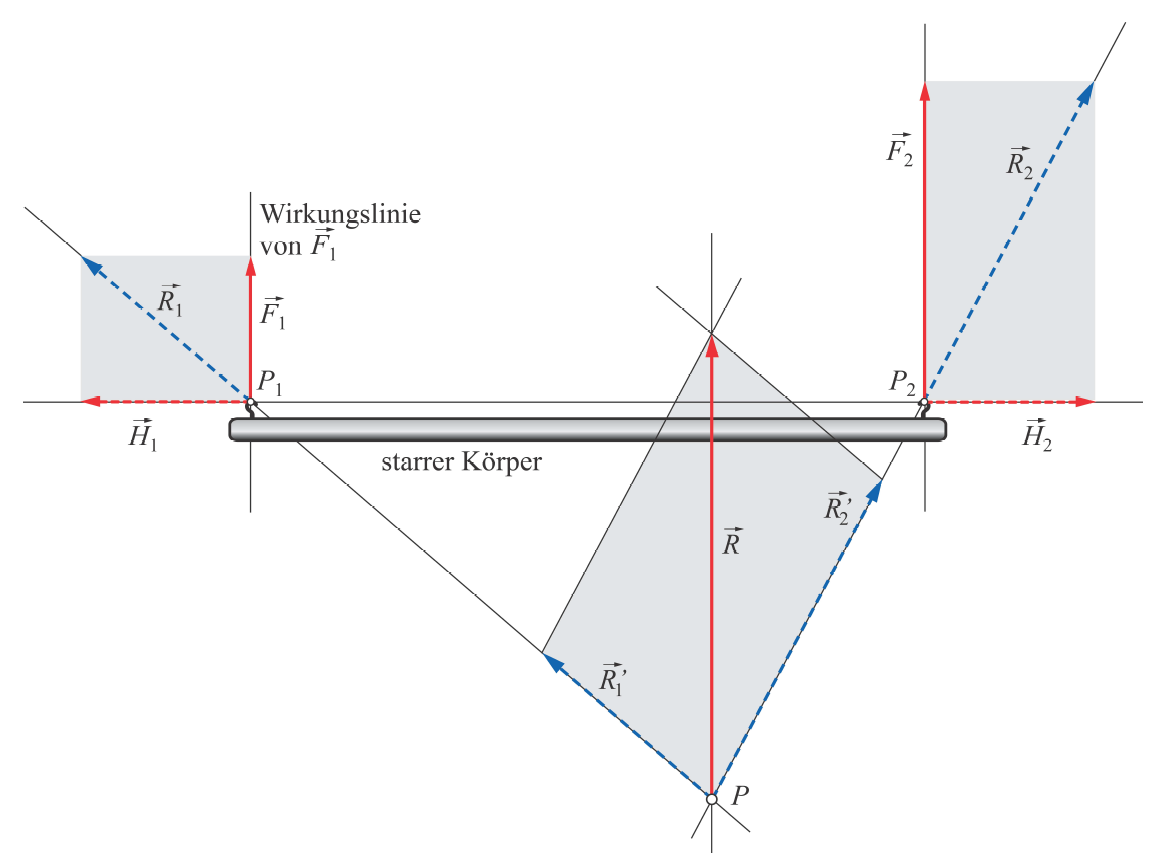
\includegraphics[width=0.7\linewidth]{Bilder/parallele_wirkungslinien}

		\subsubsection{Spezialfall: Ebene Kräftegruppe für parallel, entgegengesetzt und gleich grosse Kräfte}
	
			Kräftepaare können in andere Kräftepaare umgewandelt  werden, aber \underline{niemals zu einer} resultierenden Kraft $\vec{R}$ vereinfacht werden. \\
			\\
			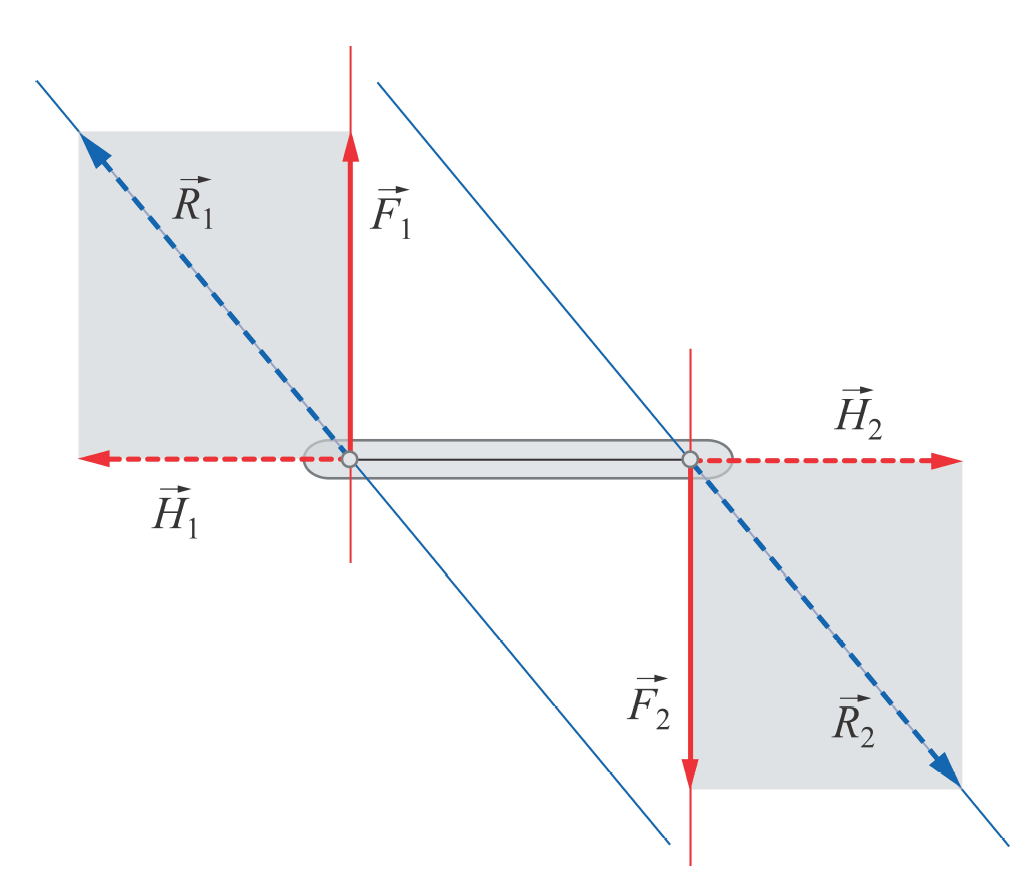
\includegraphics[width=0.7\linewidth]{Bilder/kraeftepaar_wirkungslinien}
		
	\subsection{Drehmoment}
		Eine Drehwirkung auf einen starren Körper lässt sich auf zwei \\
		verschiedene Arten und Weisen erzeugen: \\
		\\
		\begin{tabular}{ll}
			$\bullet$ & Kräftepaar \\
			$\bullet$ & einzelne Kraft und Bezugspunkt (Drehzentrum) \\
		\end{tabular}
		
		\begin{minipage}{0.48\linewidth}
			\begin{tikzpicture}
				[
				x=1cm, y=1cm, scale=0.5, font=\footnotesize, >=latex 
				%Voreinstellung für Pfeilspitzen
				]
				%Raster im Hintergrund
				%\draw[step=1, gray, very thin] (-5.5,-5.5) grid (5.5,5.5);
				\draw[thick, gray] (0, 0) circle(3.5);
				\draw[dashed] (2,3.5) -- (2,-3.5) node [midway, left, yshift=-1.2cm] {$Wirkungslinie$};
				\draw[-latex, draw=blue!50!black, very thick, rotate = -90] (1,0)--(1,0) arc(0:-250:1) 
								node [midway, above, xshift=-1.3pt, yshift=0, blue!50!black] {$\vec{M}$} {};
				\fill[black] (0, 0) circle(3.5pt) node [midway, above, yshift=7pt] {$Drehachse$};
				\begin{scope}[xshift=2cm, yshift=0cm, rotate=0, scale=1]
					%Kräfte
					\draw [-latex, very thick, green!50!black] (0,0) -- ++(0,-2) node[midway, left] {$\vec{F}{'}$};
					\fill [blue!70!white](0,0) circle (0.1) node[midway, right] {$P'$};;
				\end{scope}		
				\begin{scope}[xshift=2cm, yshift=0cm, rotate=90, scale=1]  		
					\draw [thick](-0.3,0) -- (-0.3,0.3) -- (0,0.3);
				\end{scope}	
				\begin{scope}[xshift=2cm, yshift=2.87228cm, rotate=0, scale=1]
					%Kräfte
					\draw [-latex, very thick, green!50!black] (0,0) -- ++(0,-2) node[midway, left] {$\vec{F}$};
					\fill [blue!70!white](0,0) circle (0.1) node[midway, right] {$P$};;
				\end{scope}	
				\draw[-latex, very thick, red] (0,0) -- ++(2,0) node[midway, below] {$\vec{r}$};
			\end{tikzpicture}
			\\
		\end{minipage}
		\hfill
		\begin{minipage}{0.48\linewidth}
			$ \vert \vec{M} \vert = \vert \vec{r} \times \vec{F} \vert = a \cdot \vert \vec{F} \vert  $	\\
			\\
			Die Länge a muss \textbf{senkrecht} zur wirkenden Kraft sein!
		\end{minipage}

		\begin{tabular}{lll}
			$\vec{M}$ & Drehmoment & $[M] = \mathrm{Nm}$ \\
			$\vec{r}$ & Abstandsvektor & $[r] = \mathrm{m}$ \\
			$\vec{F}$ & Angreifende Kraft & $[F] = \mathrm{N}$ \\
		\end{tabular}

	\subsection{Gleichgewichtsbedungungen für starre Körper}
		
		$ \sum \limits_{i = 1}^n \vec{F}_i = \vec{0}$  \qquad  $ \sum \limits_{i = 1}^m \vec{M}_i = \vec{0} $  \qquad $\Rightarrow$ komponentenweise
	
	\subsection{Gleichgewichts-Arten}	
		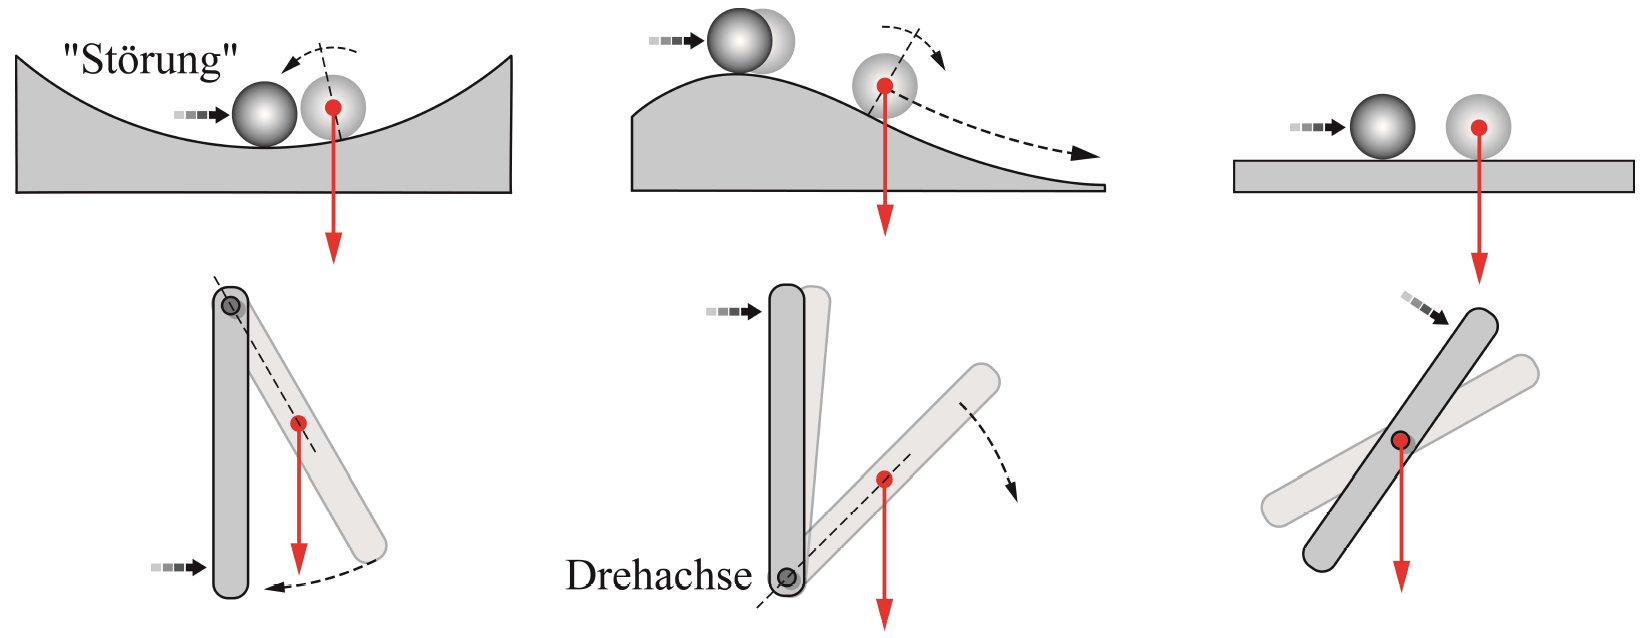
\includegraphics[width=0.95\linewidth]{Bilder/gleichgewichte} \\
		\\
		\begin{minipage}{0.3\linewidth}
			\center{stabil}
		\end{minipage}
		\hfill
		\begin{minipage}{0.3\linewidth}
			\center{labil}
		\end{minipage}
		\hfill
		\begin{minipage}{0.3\linewidth}
			\center{indifferent}
		\end{minipage}

	\subsection{Deformierbare Körper}
		
		\subsubsection{Spannungen}
			\textbf{Zugspannung $\sigma$} \\
				\\
				senkrecht wirkende Kraft pro Flächeneinheit \\
				Wenn $\sigma < 0$ spricht man von \textbf{Druck} 
				
				$$ \boxed{ \sigma = \frac{F_{\perp}}{A} } \qquad [\sigma] = \mathrm{\frac{N}{m^2}}$$ 

			\textbf{Schubspannung $\tau$ (Scherung)} \\
				\\
				parallel wirkende Kraft pro Flächeneinheit 
				
				$$ \boxed{ \tau = \frac{F_{\shortparallel}}{A} } \qquad [\tau] = \mathrm{\frac{N}{m^2}}$$

		\subsubsection{Dehnung $\epsilon$ (Hook'sches Gesetz)}
			$$ \boxed{ \epsilon = \frac{1}{E} \cdot \sigma = \frac{1}{E} \cdot \frac{F_{\perp}}{A} = \frac{\Delta \, l}{l} } $$ 

			\begin{tabular}{c l c}
				$\epsilon$ & Dehnung & $[\epsilon] = 1$ \\
				$E$ & Elastizitätsmodul (Materialeigenschaft) & $[E] = \mathrm{\frac{N}{m^2}}$ \\
				$l$ & Länge des Körpers vor Dehnung & $[l] = \mathrm{m}$ \\
				$\Delta \, l$ & Längenunterschied bei Dehnung & $[\Delta \, l] = \mathrm{m}$ \\
				$\sigma$ & Zugspannung & $[\sigma] = \mathrm{N}$ \\
				$A$ & Querschnittsfläche & $[A] = \mathrm{m^2}$ \\
				\\
			\end{tabular}
			
			$\Rightarrow$ \textbf{Das Hook'sche Gesetz gilt nur, solange die Deformation linear-elastisch ist!}

			%todo: Bild von Elastizität finden und einfügen

		\subsubsection{Querkontraktion $\epsilon_q$}
			Wird ein Stab gedehnt (länger), so wird er automatisch auch dünner \\		
			
			$$ \boxed{ \epsilon_q = \frac{\Delta \, d}{d} = - \mu \, \epsilon } \qquad \mu \in (0 \, ; \, 0.5)$$ \\
			
			\begin{tabular}{c l c}
				$\epsilon_q$ & Querkontraktion & $[\epsilon_q] = 1$ \\
				$d$ & Ursprüngliche Dicke des Materials & $[d] = \mathrm{m}$ \\
				$\Delta d$ & Dicken-Änderung & $[ \Delta \, d] = \mathrm{m}$ \\
				$\epsilon$ & (Längs-) Dehnung & $[\epsilon] = 1$ \\
				$\mu$ & Poisson-Zahl (Materialeigenschaft) & $[\mu] = 1$ \\
			\end{tabular}
		
		\subsubsection{Kompression $\frac{\Delta \, V}{V}$}
			Ein Körper wird von allen Seiten mit dem gleichen Druck belastet, sodass sich sein Volumen verkleinert 
			
			$$ \boxed{ \frac{\Delta \, V}{V} = - \kappa \cdot \Delta \, p } \qquad \Big( K = \frac{1}{\kappa} \Big) $$ \\ 
			
			\begin{tabular}{c l c}
				$V$ & Ursprüngliches Volumen des Körpers & $[V] = \mathrm{m^3}$ \\
				$\Delta V$ & Volumenänderung & $[\Delta V] = \mathrm{m^3}$ \\
				$\kappa$ & Kompressibilität & $[\kappa] = \mathrm{\frac{m^2}{N}}$ \\
				$\Delta \, p$ & Druckänderung & $[\Delta \, p] = \mathrm{\frac{N}{m^2} = Pa}$  \\ 
			\end{tabular}
			
			$$ \boxed{ \text{Würfel:} \quad \Rightarrow \kappa = \frac{3}{E} (1 - 2 \, \mu) }$$ 
			
			\textbf{Völlig inkompressibler Körper:} $\kappa = 0$  \qquad $K = \infty$ \qquad $\mu = 0.5$

		\subsubsection{Schubbeanspruchung (Scherung)}
		
			$$ \boxed{ \gamma = \frac{1}{G} \, \tau }$$ 
			
			$$ \boxed{ G = \frac{E}{2(1 + \mu)}  \quad \text{(gilt für isotrope Materialen)} } $$\\

			\begin{tabular}{c l c}
				$\gamma$ & Scherwinkel & $[\gamma] = \; ^\circ $ \\
				\rule{0pt}{10pt}$G$ & Schubmodul; Gleitmodul; Torsionsmodul & $[G] = \mathrm{\frac{N}{m^2}}$ \\
				\rule{0pt}{10pt}$\tau$ & Schubspannung & $[\tau] = \mathrm{\frac{N}{m^2}}$ \\
				\rule{0pt}{10pt}$E$ & Elastizitätsmodul (Materialeigenschaft) & $[E] = \mathrm{\frac{N}{m^2}}$ \\
				$\mu$ & Poisson-Zahl (Materialeigenschaft) & $[\mu] = 1$ \\
			\end{tabular}

		\subsubsection{Torsionsfeder}
		
			$$ \boxed{ M = c \cdot \varPhi \quad \quad c = \frac{\pi G r^4}{2l} }$$ 

			\begin{tabular}{c l c}
				$M$ & Drehmoment & $[M] = Nm$ \\
				$c$ & Auslenkkonstante & $[c] = $ \\
				$\varPhi$ & Auslenkwinkel & $[\varPhi] = \; ^\circ $ \\
				$G$ & Schubmodul & $[G] = \mathrm{\frac{N}{m^2}}$ \\
				$r$ & Radius der Feder & $[r] = m$ \\
				$l$ & Länge der Feder & $[l] = m$ \\
			\end{tabular}

		\subsubsection{Schraubenfeder}
		
			$$ \boxed{ F = c \cdot \Delta l \quad \quad c = \frac{G r^4}{4nR^3} }$$ 

			\begin{tabular}{c l c}
				$F$ & Kraft & $[F] = N$ \\
				$c$ & Auslenkkonstante & $[c] = $ \\
				$\Delta l$ & Längenänderung & $[\Delta l] = m$ \\
				$G$ & Schubmodul & $[G] = \mathrm{\frac{N}{m^2}}$ \\
				$r$ & Drahtradius der Feder & $[r] = m$ \\
				$R$ & Windungsradius der Feder & $[R] = m$ \\
				$n$ & Anzahl Windungen & $[n] = $ \\
			\end{tabular}

		\subsubsection{Blattfeder}
		
			$$ \boxed{ z = \frac{4l^3}{E \cdot b \cdot h^3}F }$$ 

			\begin{tabular}{c l c}
				$F$ & Kraft & $[F] = N$ \\
				$z$ & Verbiegung & $[z] = m$ \\
				$l$ & Längenänderung & $[l] = m$ \\
				$E$ & Elastizitätsmodul & $[E] = \mathrm{\frac{N}{m^2}}$ \\
				$b$ & Breite des Querschnitts & $[b] = m$ \\
				$h$ & Höhe des Querschnitts & $[h] = m$ \\
			\end{tabular}

	\subsection{Schiefe Ebene (mit Seil)}
		\begin{tikzpicture}
			[
			x=1cm, y=1cm, scale=0.85, font=\footnotesize, >=latex 
			%Voreinstellung für Pfeilspitzen
			]
			
			%Raster im Hintergrund
			%\draw[step=1, gray, very thin] (0,0) grid (7,6);	

			%Grunddreieck	
			\draw [fill=gray!20] (0,0) -- (7,0) -- (7,4.04145) -- (0,0);
			
			%Winkel
			\filldraw[fill=blue!10, draw=blue!50!black, thick] (0,0) -- (1.5,0) arc(0:30:1.5) 
				node [midway, xshift=-10pt, yshift=-3, blue!50!black] {$\alpha$} {};
					
			\draw [very thick] (0,0) -- (7,0) -- (7,4.04145) -- (0,0);
					
			%Bezugssystem
			\begin{scope}[xshift=1cm, yshift=3cm, rotate=30, scale=1]
				%Länge x Achse
				\draw [-latex, thick] (0,0) -- ++(1,0) node[below, rotate=30] {$x$};
			
				%Länge y Achse
				\draw [-latex, thick] (0,0) -- ++(0,1) node[left, rotate=30] {$y$};
			\end{scope}
			%Alles was gedreht wurde (Masse m, Kräftevektoren, ...)
			\begin{scope}[xshift=3.464cm, yshift=2cm, rotate=30, scale=1.1]

				\coordinate (A) at (0.75,0.5);
				\coordinate (B) at (0.75,-1.5);
				
				%Rechteck
				\draw [fill=orange!20!white] (0,0) rectangle (1.5,1);
				\draw [orange, very thick] (0,0) rectangle (1.5,1) node [midway, right, xshift=3pt, yshift=3pt] {$m$} {} ;
				
				%Vektoren Kraft-Seil
				\begin{scope}[xshift=1.5cm, yshift=1cm, rotate=0, scale=1]
					\begin{scope}[xshift=0cm, yshift=0cm, rotate=0, scale=1]
						\filldraw[fill=green!10, draw=green!50!black, thick] (0,0) -- (1,0) arc(0:33.6900:1) 
							node [midway, left, xshift=0pt, yshift=-7, green!50!black] {$\beta$} {};
					\end{scope}
					\coordinate (C) at (1.5,0);
					\coordinate (D) at (1.5,1);
					%Rechter Winkel
					\draw [thick](1.2,0) -- (1.2,0.3) -- (1.5,0.3);
					\draw [-latex, very thick, purple] (0,0) -- ++ (C) node [midway, below] {$\vec{F}_{Sx}$} {};
					\draw [-latex, very thick, green!50!black] (C) -- ++ (0,1) node [midway, right] {$\vec{F}_{Sy}$} {};
					\draw [-latex, very thick, red] (0,0) -- ++ (D) node [midway, left] {$\vec{F}_S$} {};
					%Rechter Winkel
				
				\end{scope}	
				
				%Vektoren FN, FG, FH
				
				\begin{scope}[xshift=0cm, yshift=0, rotate=0, scale=1]
					\coordinate (A) at (0.75,0.5);
					\coordinate (B) at (0.75,-1.5);
					\begin{scope}[xshift=0.75cm, yshift=0.5cm, rotate=-120, scale=1]
						\filldraw[fill=blue!10, draw=blue!50!black, thick] (0,0) -- (1,0) arc(0:30:1) 
							node [midway, above, xshift=-1.5pt, yshift=0, blue!50!black] {$\alpha$} {};
					\end{scope}
					%Rechter Winkel
					\draw [thick](0.45,-1.5) -- (0.45,-1.2) -- (0.75,-1.2);  
					\draw [-latex, very thick, dashed, green!50!black] (B) -- (A) node [midway, right] {$\vec{F}_N$} {};
					\draw [-latex, very thick, green!50!black] (A) -- ++(0,2) node [midway, right] {$\vec{F}_N$} {};
					\draw [-latex, very thick, purple] (B) -- ++(-1.1547,0) node [midway, below] {$\vec{F}_H$} {};
					\draw [-latex, very thick, red] (A) -- ++(-1.1547,-2) node [midway, left] {$\vec{F}_G$} {};
					%Rechter Winkel
					\draw [thick](0.45,-1.5) -- (0.45,-1.2) -- (0.75,-1.2);  
				\end{scope}		    		
			\end{scope}
			
		\end{tikzpicture}
		\\
		\textbf{Wichtige Formeln und Zusammenhänge zur schiefen Ebene} \\
			\\
			\begin{tabular}{lll}
				$F = m \cdot a$  & $F_G = m \cdot g$ \\
				\\
				$F_N = m \cdot g \cdot \cos(\alpha)$ & 
				$F_H = m \cdot g \cdot \sin(\alpha)$ \\
			\end{tabular}

	\subsection{Rezept: Aufgaben zur Statik lösen}
	
	\begin{tabular}{ll}
		1. & Koordinatensystem festlegen  \\
		2. & Alle wirkenden Kräfte einzeichnen \\
		3. & Bezugspunkt P (Drehpunkt) festlegen \\
		& $\Rightarrow$ \textbf{Da wo viele Kräfte} (oder da wo sinnvoll) \\
		4. & Kräfte komponentenweise aufschreiben: $\sum \vec{F}_i = 0$ \\
		5. & Drehmomente M aufschreiben und gleichsetzen: $\overleftarrow{M} = \overrightarrow{M}$ \\
	\end{tabular}

	\vfill\null
	\pagebreak
		
		%Code geputzt, Inhalt kontrolliert

		\section{Kinematik}
			
	\subsection{Geradlinige Bewegung (1D)}
		Die Bewegung erfolgt entlang einer Gerade (keine Richtungsänderung) \\
		\\
		\begin{minipage}{0.48\linewidth}
			\begin{equation*}
				x(t) \quad  \underrightarrow{ \frac{d}{dt}} \quad  v(t) \quad  \underrightarrow{ \frac{d}{dt}} \quad a(t)  
			\end{equation*}
		\end{minipage}
		\hfill
		\begin{minipage}{0.48\linewidth}
			\begin{equation*}
				x(t) \quad \underleftarrow{\int dt} \quad v(t) \quad \underleftarrow{\int dt} \quad a(t)
			\end{equation*}
		\end{minipage}

		\subsubsection{Weg $x(t)$}
			Weg mit Zeit parametrisiert: $x = x(t)$ 

		\subsubsection{Geschwindigkeit $v(t) = \frac{\Delta \, x}{\Delta \, t}$}
		
			\begin{tabular}{lll}
				momentane Geschw.: & $\frac{d}{dt} x(t) = \dot{x}(t)$ & (Tangente) \\	
				\\
				mittlere Geschw.: & $\overline{v} = \frac{x_2 -x_1}{t_2 - t_1} =  \frac{x(t_2) - x(t_1)}{t_2 - t_1} $  & (Sekante) \\
			\end{tabular}

		\subsubsection{Beschleunigung $a(t) = \frac{\Delta \, v}{\Delta \, t}$}
			
			\begin{tabular}{ll}
				momentane Beschleunigung: & $\frac{d}{dt} v(t) = \dot{v}(t) = \ddot{x}(t)$ \\	
				\\
				mittlere Beschleunigung: & $\overline{a} = \frac{v_2 -v_1}{t_2 - t_1} =  \frac{v(t_2) - v(t_1)}{t_2 - t_1} $ \\
			\end{tabular}

		\subsubsection{Ruck $j(t)$}
		Änderung der Beschleunigung pro Zeiteinheit: $j(t) = \dot{a}(t) = \dddot{x}(t)$

	\subsection{Gleichförmige Bewegung $a(t) = 0$}
		\begin{tabular}{l}
			$a(t) = 0$ \\
			\\
			$v(t) = v_0 = \; \text{const}$ \\
			\\
			$x(t) = v_0 \cdot t + x_0 $ \\
		\end{tabular}
		
	\subsection{Gleichm. beschleunigte Bewegung $a(t) = $ konst}
		\begin{minipage}{0.48\linewidth}
			\textbf{Allgemein:} \\
				\\
				\begin{tabular}{l}
					$a(t) = a_0 = \text{const}$ \\
					\\
					$v(t) = a_0 \cdot t + v_0$ \\
					\\
					$x(t) = \frac{1}{2} \, a_0 \cdot t^2 + v_0 \cdot t + x_0$
				\end{tabular}
		\end{minipage}
		\hfill
		\begin{minipage}{0.48\linewidth}
			\textbf{Anwendungsfall: Freier Fall} \\
				\\
				\begin{tabular}{ll}
					$a(t) = -g = \text{const}$ \\
					\\
					$v(t) = -g \cdot t $ \\
					\\
					$x(t) = - \frac{1}{2} \, g \cdot t^2 + h_0$
				\end{tabular}
		\end{minipage}

		\subsubsection{Höchsten Punkt $x_{max}$ finden (Extremum)}
		
			Im Extremalpunkt gilt: $\frac{d}{dt} x(t) = v(t) \overset{!}{=} 0$ \\
			\\
			$0 \overset{!}{=} v(t_{max}) = -g \cdot t_{max} + v_0 $ \qquad \qquad $\Rightarrow t_{max} = \frac{v_0}{g}$ \\
			
			Durch einsetzen von $t_{max}$ in $x(t)$ erhält man die maximale Höhe: \\
			$x(t_{max}) = - \frac{1}{2}\, g \cdot t_{max}^2 + v_0 \cdot t_{max} + h_0 = - \frac{v_0^2}{2 \, g}\, + \frac{v_0^2}{g} + h_0 $

	\subsection{Beliebige Bewegung (2D)}
		
		\subsubsection{Geschwindigkeit (tangential zur Bahnkurve)}
		
			\begin{tabular}{ll}
				momentane Geschw.: & $ \vec{v} = \lim \limits_{\Delta t \rightarrow 0} \frac{\Delta \vec{r}}{\Delta t}  \frac{d}{dt} \vec{r} = \dot{\vec{r}}$ \\	
				\\
				mittlere Geschw.: & $\overline{\vec{v}} = \frac{\Delta \vec{r}}{\Delta t} = \frac{\vec{r}(t + \Delta t) - \vec{r}(t)}{\Delta t} $ \\
				\\
				Betrag: & $v = \vert \vec{v} \vert = \lim \limits_{\Delta t \rightarrow 0} \frac{ \vert \Delta \vec{r} \vert}{\Delta t} = \lim \limits_{\Delta t \rightarrow 0} \frac{\Delta s }{\Delta t} = \frac{d}{dt} s$ \\
			\end{tabular}

		\subsubsection{Beschleunigung}
			\begin{tabular}{ll}
				momentane Beschl.: & $ \vec{a} = \frac{d}{dt} \vec{v} = \dot{\vec{v}} = \frac{d^2}{d t^2} \vec{r} = \ddot{\vec{r}}$ \\	
				\\
				mittlere Beschl.: & $\overline{\vec{a}} = \frac{\Delta \vec{v}}{\Delta t} $ \\
			\end{tabular}
		
			\textbf{Die Beschleunigung kann ungleich null sein, auch wenn der Betrag der Geschwindigkeit konstant ist}

	\subsection{Bahnkurven}	
		Die Geschwindigkeitsänderung in einer Bahnkurve wird in zwei \\
		Komponenten aufgeteilt: \\
			$\Delta \vec{v}_{radial}$ \quad und \quad $\Delta \vec{v}_{tangential}$ \\
			\\
		Der tangentiale Anteil ändert ausschliesslich den Betrag der \\
		Geschwindigkeit $\vert \vec{v} \vert$ \\
		Der radiale Anteil ändert ausschliessich die Richtung der \\
		Geschwindigkeit $\vec{v}$ \\

		\begin{minipage}{0.45\linewidth}
			\begin{tikzpicture}
				[
				x=1cm, y=1cm, scale=0.6, font=\footnotesize, >=latex 
				%Voreinstellung für Pfeilspitzen
				]
				%Raster im Hintergrund
				%\draw[step=1, gray, very thin] (0,0) grid (5.5,5.5);
				\draw[thick] (0, 0) circle(2.5);
				\fill[black] (0, 0) circle(5pt) node [midway, above, yshift=7pt, scale=2] {$m$};
				\begin{scope}[xshift=2.5cm, yshift=0cm, rotate=0, scale=1]
					%Kräfte
					\draw [-latex, very thick, green!50!black] (0,0) -- ++(0,-2) node[midway, right, scale=1.2] {$\vec{a}_{tangential}$};
					\draw [-latex, very thick, purple] (0,0) -- ++(-1.5,0) node[midway, above, scale=1.2, xshift=-3pt] {$\vec{a}_{radial}$};
					\draw [-latex, very thick, orange] (0,0) -- ++(-1.5,-2) node[midway, left, scale=1.2] {$\vec{a}_{tot}$};
					\fill [blue!70!white](0,0) circle (0.1) node[midway, right, scale=2] {$P$};;
				\end{scope}		
			\end{tikzpicture}
		\end{minipage}
		\hfill
		\begin{minipage}{0.55\linewidth}
			$a_{tangential} = \frac{dv}{dt} = \dot{v}$ \\
			\\
			$a_{radial} = \frac{v^2}{r}$ \\
			\\
			$ \boxed { F_{zentripetal} = m \, \frac{v^2}{r} }$ \\
			\\
			$ \boxed{ (F_{zentri})^2 + (F_{bremsen})^2 = (F_R)^2 }$
		\end{minipage}

	\subsection{Gleichförmige Bewegung $a_{tangential} = 0$}
	
		\begin{minipage}{0.6\linewidth}
			\textbf{tangential (Tacho)} \\
				\\
				$a_{tangential} = 0$ \\
				\\
				$v(t) = v_0 = \text{const}$ \\
				\\
				$s(t) = v_0 \cdot t + s_0$ \\
		\end{minipage}
		\hfill
		\begin{minipage}{0.35\linewidth}
			\textbf{radial} \\
				\\
				$a_{radial} = \frac{v^2}{r}$ \\
				\\
				\\
				\\
				\\
		\end{minipage}

	\subsection{Gleichm. beschl. Bewegung $a_{tangential} = \text{konst}$}		
		\begin{minipage}{0.6\linewidth}
			\textbf{tangential (Tacho)} \\
				\\
				$a_{tangential} = a_0 = \text{const}$ \\
				\\
				$v(t) = a_{tangential} \cdot t + v_0 $ \\
				\\
				$s(t) = \frac{1}{2} \, a_{tangential} \cdot t^2 +  v_0 \cdot t + s_0$ \\
		\end{minipage}
		\hfill
		\begin{minipage}{0.35\linewidth}
			\textbf{radial} \\
				\\
				$a_{radial} = \frac{v^2}{r}$ \\
				\\
				\\
				\\
				\\
		\end{minipage}

		Die Gesamtbeschleunigung eines Systems $\vec{a}_{tot} = \vec{a}_{tangential} + \vec{a}_{radial} $ muss nicht zwingend konstant sein! Bei Änderungen der Richtung ändert die Gesamtbeschleunigung. 
	
	\subsection{Kreisbewegung}
		
		\subsubsection{Winkel $\phi$ (zurückgelegter Weg)}
		
		\begin{minipage}{0.5\linewidth}
			\begin{tikzpicture}
				[
				x=1cm, y=1cm, scale=1.0, font=\footnotesize, >=latex 
				%Voreinstellung für Pfeilspitzen
				]

				%Länge x Achse
				\draw [thick] (0,0) -- ++(2,0) node[below] {};
				\draw [thick] (1,0) node[below] {$r$};
				
				%Zahlen auf x-Achse
				\foreach \x in {0,2}
				\draw[shift={(\x,0)},color=black, thick] (0pt,2pt) -- (0pt,-2pt);
				
				%Winkelgugus
				\begin{scope}[xshift=0cm, yshift=0.25cm, rotate=0, scale=1]
					\filldraw[fill=white, thick] (0,0) -- (2,0) arc (0:30:2) -- cycle 
						node[midway, below, green!50!black, xshift=0pt, yshift=0pt] {};
					\filldraw[fill=white, thick] (0,0) -- (1,0) arc (0:30:1) -- cycle 
						node[midway, xshift=8pt, yshift=-1pt] {$\phi$};
				\end{scope}
				
				\draw [<->, thick] (2.25,0.25) arc (0:30:2.25) node[midway, right, xshift=0pt, yshift=0pt] {$S$};
			\end{tikzpicture}
		\end{minipage}
		\hfill
		\begin{minipage}{0.4\linewidth}
			$\boxed{ \text{Radiant: } \phi = \frac{s}{r} }$ 
		\end{minipage}

		\subsubsection{Winkelgeschwindigkeit $\omega= \frac{\phi}{t}$}
		
			$\omega := \lim \limits_{\Delta t \rightarrow 0} \frac{\phi(t + \Delta t) - \phi(t)}{\Delta t} = \frac{d \phi}{dt} = \dot{\phi}$ \\
			\\
			Der Betrag $v$ der (Bahn-) Geschwinndigkeit entspricht: $v = r \cdot \omega$ \\

			\begin{tabular}{ll}
				Umlaufzeit, Periode $T$ & Umlaufzeit für vollständige Umdrehung \\
				\\
				Drehzahl, Drehfrequenz $f$ & inverse Umlaufzeit   $f = \frac{1}{T}$ \\
				\\
				\\
			\end{tabular}
			
			\textbf{Wichtige Umrechnungsformeln} \\		 
				\\
				\boxed{
					\begin{tabular}{l c l l}
						$v = r \cdot \omega$ & $\Leftrightarrow$ & $\omega = \frac{v}{r}$ & \\		
						\\
						$f = \frac{1}{T}$ & $\Leftrightarrow$ & $T = \frac{1}{f}$ & \\
						\\
						$\omega = \frac{2 \, \pi}{T}$ & $\Leftrightarrow$ & $T = \frac{2 \, \pi}{f}$ & $\omega = \frac{2 \pi n}{60} $ \\
						\\
						$\omega = 2 \, \pi \, f$ & $\Leftrightarrow$ & $f = \frac{\omega}{2 \, \pi} $ & $v = \frac{\pi d n}{60} $ \\
					\end{tabular}
				}

		\subsubsection{Winkelbeschleunigung $\alpha = \frac{\omega}{t}$}
		
			$\alpha = \lim \limits_{\Delta t \rightarrow 0} \frac{\omega(t + \Delta t) - \omega(t)}{\Delta t} = \frac{d \omega}{dt} = \dot{\omega} = \frac{d^2 \, \phi}{d t^2} \ddot{\phi} $ \\
			\\
			$a_{tangential} = \frac{dv}{dt} = \frac{d}{dt} r \cdot \omega = r \cdot \alpha$

	\subsection{Gleichförmige Kreisbewegung}
		
		\begin{tabular}{l}
			$\alpha(t) = 0$ \\
			\\
			$\omega(t) = \omega_0 = \text{const}$ \\
			\\
			$\phi(t) = \omega_0 \, t + \phi_0$ 
		\end{tabular}

	\subsection{Gleichm. beschleunigte Kreisbewegung}
		
		\begin{tabular}{l}
			$\alpha(t) = \alpha_0 = \text{const} $ \\
			\\
			$\omega(t) = \alpha_0 \cdot t + \omega_0$ \\
			\\
			$\phi(t) = \frac{1}{2} \, \alpha_0 \cdot t^2 + \omega_0 \cdot t + \phi_0$ \\
		\end{tabular}

	\subsection{Senkrechter Wurf}

		\begin{minipage}{0.45\linewidth}
			\begin{tikzpicture}
				[
				x=1cm, y=1cm, scale=0.5, font=\footnotesize, >=latex 
				%Voreinstellung für Pfeilspitzen
				]
				
				%Raster im Hintergrund
				%\draw[step=1, gray!50!white, very thin] (-2,-2) grid (5,5);
				
				%Zahlen auf x-Achse
				\foreach \x in {-0.75,0.25,1.25,2.25,3.25,4.25}
				\draw[shift={(\x,0)},color=gray, very thick] (0pt,0pt) -- (-10pt,-10pt);
				
				\draw [very thick] (0.5,0)--(0,1);
				\draw [very thick] (-0.5,0)--(0,1);
				\draw [very thick] (0,1)--++(0,1);
				\draw [very thick] (0,1.75)--(0.5,1.55)--(1,1.75);
				\fill (0,2.35) circle (0.35);
				\fill [orange](1,1.75) circle (0.15);

				%Länge x Achse
				\draw [thick] (-1,0) -- ++(5.5,0);
				\draw [-latex, very thick, red] (1,1.75)--++(0,1.5) node [midway, right, red, xshift=0pt, yshift=0pt, scale=1.5] {$\vec{v}_0$} {};
				\draw [-latex, very thick, gray] (4,4)--++(0,-1.5) node [midway, left, gray, xshift=0pt, yshift=0pt, scale=1.5] {$-\vec{g}$} {};
				\draw [-latex, very thick] (-1,0)--++(0,4) node [above, xshift=0pt, yshift=0pt, scale=1.5] {$y$} {};
				\draw [<->, very thick, gray] (2,0)--++(0,1.75) node [midway, right, gray, xshift=0pt, yshift=0pt, scale=1.5] {$h_0$} {};
				\draw [dashed, thick] (1,1.75)--++(1,0);
			\end{tikzpicture}
		\end{minipage}
		\hfill
		\begin{minipage}{0.5\linewidth}
			$a = -g = \text{const}$ \\
			\\
			$v(t) = -g \cdot t + v_0$ \\
			\\
			$h(t) = - \frac{1}{2} \, g \cdot t^2 + v_0 \cdot t + h_0$ \\
		\end{minipage}

		\subsubsection{Maximale Flughöhe $h_{max}$ bestimmen}
			Bei der maximalen Flughöhe $h_{max}$ gilt: $v(t) \overset{!}{=} 0$ \\
			\\
			$v_0 - g \cdot t_{max} \overset{!}{=} 0$ \qquad $\Rightarrow$ \qquad $t_{max} = \frac{v_0}{g}$ \\
			\\
			Nun wird $t_{max}$ in $h(t)$ eingesetzt: \\
			\\
			$h_{max} = h(t_{max}) = - \frac{g}{2} \, \frac{v_0^2}{g^2} + v_0 \, \frac{v_0}{g} + h_0 = \frac{v_0^2}{2 \, g} + h_0 $ \\
			\\
			\\
			\textbf{Hinweis: Die maximale Flughöhe kann auch über die potentielle und kinetische Energie berechnet werden!} \\
				$E_{kin} \overset{!}{=} 0 $ \qquad $E_{pot} \overset{!}{=} m \cdot g \cdot h_{max} $ \\
				$\frac{1}{2} \, m \cdot v^2 = m \cdot g \cdot h_{max}$ \quad $\Rightarrow$ \quad $h_{max} = \frac{m \, v^2}{2 \, m  \, g} =  \frac{v^2}{2 \, g} $  \\
				\\
				$\Rightarrow$ für \underline{abgeschlossene} Systeme!
			
\vfill\null
\columnbreak
	
	\subsection{Horizontaler Wurf}
	
		\begin{tikzpicture}
			[
			x=1cm, y=1cm, scale=0.5, font=\footnotesize, >=latex 
			%Voreinstellung für Pfeilspitzen
			]
			
			%Raster im Hintergrund
			\draw[,step=1, gray!50!white, very thin] (0,0) grid (9.5,7.5);
			
			%Länge x-Achse
			\draw [-latex, very thick] (0,0) -- ++(9.5,0) node[below, scale=1.5] {$x$};
			
			%Länge y-Achse
			\draw [-latex, very thick] (0,0) -- ++(0,7.5) node[left, scale=1.5] {$y$};
			
			%Zahlen auf y-Achse 
			\foreach \y in {0,1,2,3,4,5,6,7}
			\draw[shift={(0,\y)}, color=black, thick] (2pt,0pt) -- (-2pt,0pt);
			
			%Zahlen auf x-Achse
			\foreach \x in {0,1,2,3,4,5,6,7,8,9}
			\draw[shift={(\x,0)},color=black, thick] (0pt,2pt) -- (0pt,-2pt);
			
			\draw [] (0,6) node[gray, left, scale=1.5] {$y_{0}$};	
			\draw [] (8,0) node[orange, below, scale=1.5] {$x_{max}$};	
			\fill [orange] (8,0) circle (0.1);
			% die Parable halt
			\draw[green!50!black, very thick] (0,6) parabola bend (0,6) (8,0);			

			%Vektor v0
			\fill [red] (0,6) circle (0.1);
			\draw[-latex, very thick, red] (0,6) -- ++ (2,0) node [midway, above, red, xshift=7pt, yshift=0pt, scale=1.5] {$\vec{v}_0=\vec{v}_x$} node (v) {};		
			
			%Vektor v1
			\fill [red] (4,4.5) circle (0.1);
			\draw[-latex, very thick, red] (4,4.5) -- ++ (2,0) node [midway, above, red, xshift=0pt, yshift=0pt, scale=1.5] {$\vec{v}_x$} node (v) {};
			\draw[-latex, very thick, red] (4,4.5) -- ++ (0,-1.495) node [midway, left, red, xshift=-4pt, yshift=-1pt, scale=1.5] {$\vec{v}_y$} {};
			\draw[-latex, very thick, blue] (4,4.5) -- ++ (2,-1.495) node [midway, below, blue, xshift=0.9cm, yshift=0pt, scale=1.5] {$\vec{v}_r$} {};
			\draw [dashed, gray, thick] (4,3)--(6,3)--(6,4.5);
			
			\draw [-latex, very thick] (9,7)--(9,5.5) node [midway, left, xshift=0cm, yshift=0pt, scale=1.5] {$-\vec{g}$} {};
		\end{tikzpicture}

		Der horizontale Wurf muss komponentenweise beschrieben werden \\
		x-Achse: gleichförmige, unbeschleunigte Bewegung \\
		y-Achse: gleichmässig beschleunigte Bewegung \\
		
		\begin{minipage}{0.45\linewidth}
			\textbf{x-Achse} \\
				\\
				$a_x = 0$ \\
				$v_x = v_0$ \\
				$x = v_0 \cdot t + x_0$ \\
		\end{minipage}	
		\hfill	
		\begin{minipage}{0.45\linewidth}
			\textbf{y-Achse} \\
				\\
				$a_y = -g$ \\
				$v_y = -g \cdot t$ \\
				$y = - \frac{1}{2} \, g \cdot t^2 + y_0$ \\
		\end{minipage}	
		
		\textbf{Tipp:} Lege den Koordinatenursprung in den Abwurf-Ort
	
		\subsubsection{Beschreibung der Flugbahn (Eliminierung von $t$)}	
			Die y-Koordinate soll als Funktion der x-Koordinate ausgedrückt werden: $y = f(x)$ \\
			\\
			$x = v_0 \, t$ \quad $\Leftrightarrow$ \quad $t = \frac{x}{v_0}$ \quad $\Rightarrow$ \quad $y = - \frac{1}{2} \, g \cdot t^2 = - \frac{g}{2} \frac{x^2}{v_0^2} = y(x)$
			
	\subsection{Schiefer Wurf}
	
		\begin{tikzpicture}
			[
			x=1cm, y=1cm, scale=1.3, font=\footnotesize, >=latex 
			%Voreinstellung für Pfeilspitzen
			]
			
			%Raster im Hintergrund
			\draw[step=1, gray!50!white, very thin] (0,0) grid (4.5,1.5);
			
			%Länge x-Achse
			\draw [-latex] (0,0) -- ++(4.5,0) node[below] {$x$};
			
			%Länge y-Achse
			\draw [-latex] (0,0) -- ++(0,1.5) node[left] {$y$};
			
			%Zahlen auf y-Achse 
			\foreach \y in {0,1}
			\draw[shift={(0,\y)}] (2pt,0pt) -- (-2pt,0pt);
			
			%Zahlen auf x-Achse
			\foreach \x in {0,1,2,3,4}
			\draw[shift={(\x,0)},color=black] (0pt,2pt) -- (0pt,-2pt);
			
			\filldraw[fill=green!20!white, draw=green!50!black] (0,0) -- (0.75,0) arc (0:45:0.75) -- cycle node[midway, below, green!50!black, xshift=4pt, yshift=2pt] {$\phi$};
			
			%gestrichelte linie
			\draw [dashed, orange, thick] (2,0) -- (2,1);
			
			\draw [] (0,1) node[gray, left] {$h_{max}$};
			\draw [] (0,0) node[gray, left] {$h_{0}$};	
			\draw [] (0,0) node[orange, below] {$0$};
			\draw [] (4,0) node[orange, below] {$s_{max}$};	
			\draw [] (2,0) node[orange, below] {$\dfrac{s_{max}}{2}$};	
			
			% die Parable halt
			\draw[red,thick] (0,0) parabola bend (2,1) (4,0);
			
			\draw [dashed, gray, thick] (2,1)-- (0,1);		
			
			%Vektor v
			\draw[-latex, thick, blue] (0,0) -- (0.8,0.8) node [midway, above, blue, xshift=-4pt, yshift=-1pt] {$\vec{v}$} node (v) {};		
			
		\end{tikzpicture}

		Der schiefe Wurf muss komponentenweise beschrieben werden \\
		x-Achse: gleichförmige, unbeschleuigte Bewegung \\
		y-Achse: gleichmässig beschleunigte Bewegung \\
		
		\begin{minipage}{0.45\linewidth}
			\textbf{x-Achse} \\
				\\
				$a_x = 0$ \\
				$v_x = v_0 \cdot \cos(\phi)$ \\
				$x = v_0 \cdot \cos(\phi) \cdot t + x_0$ \\
		\end{minipage}	
		\hfill	
		\begin{minipage}{0.45\linewidth}
			\textbf{y-Achse} \\
				\\
				$a_y = -g$ \\
				$v_y = -g  \cdot t + v_0 \cdot \sin(\phi)$ \\
				$y = - \frac{1}{2} \, g \cdot t^2 + v_0 \cdot \sin(\phi) \cdot t + y_0$ \\
		\end{minipage}	
		
		\textbf{Tipp:} Lege den Koordinatenursprung in den Abwurf-Ort

		\subsubsection{Beschreibung der Flugbahn (Eliminierung von $t$)}	
			Die y-Koordinate soll als Funktion der x-Koordinate ausgedrückt werden: $y = f(x)$ \\
			\\
			$x(t) = v_0 \cdot \cos(\phi) \cdot t$ \quad $\Rightarrow$ \quad $t = \frac{x}{v_0 \cdot \cos(\phi)}$ \\
			\\
			$\Rightarrow$ \quad $y = - \frac{g}{2 \, v_0^2 \cdot \cos^2(\phi)} \cdot x^2 + \tan(\phi) \cdot x = y(x)$

		\subsubsection{Ansätze zur Bestimmung von Extrema}		
			\begin{tabular}{ll}
				max. Wuftweite $s_{max}$ & $y \overset{!}{=} 0 $ \quad ($\phi \in \{ 45° ; 135° \}$)\\
				& $s_{max} = x_{max} \in \{ 0, \frac{2 \, v_0^2}{g} \cos(\phi) \cdot \sin(\phi) \}$ \\
				\\
				Elevationswinkel & $\phi = \frac{1}{2} \arcsin \big( \frac{g \cdot d}{v_0^2} \big) = \frac{1}{2} \arcsin \big( \frac{g \cdot x_{max}}{v_0^2} \big)$ \\
				\\
				max. Wurfhöhe & $v_y \overset{!}{=} 0 $ \\
				& $x_{maxH"ohe} =  h_{max} = \frac{s_{max}}{2} = \frac{x_{max}}{2}$ \\
				& $y(x_{maxH"ohe}) = \frac{v_0^2 \cdot sin^2(\phi)}{2 \, g}$
			\end{tabular}

		%Code geputzt, Inhalt noch pendent

		\section{Dynamik}
		
	\subsection{Newtonsche Gesetze}
		Gesetze, welche Bewegungen beschreiben.

		\subsubsection{Erstes Newtonsches Gesetz: Trägheitsgesetz}
			Ein Körper verharrt in seine Zustand (Ruhe, gleichförmige geradlinige Bewegung), wenn er nicht durch eine Kraft gezwungen wird, seinen Zustand zu ändern. \\
			\\
			Die \textbf{Trägheit} eines Körpers hängt von seiner (Trägheits-) Masse ab.
			
		\subsubsection{Zweites Newtonsches Gesetz: Aktionsgesetz}	
			\begin{minipage}{0.2\linewidth}
				$\boxed {\vec{F} = m \cdot \vec{a} }$
			\end{minipage}
			\hfill
			\begin{minipage}{0.75\linewidth}
				\begin{tabular}{c l c}
					$\vec{F}$ & Kraft & $[F] = \mathrm{\frac{kg \cdot m}{s^2}  = N}$ \\
					$m$ & (Trägheits-) Masse & $[m] = \mathrm{kg}$ \\	
					$\vec{a}$ &  Beschleunigung & $[a] = \mathrm{\frac{m}{s^2}}$ \\
					\\
				\end{tabular}
			\end{minipage}
				
			$\Rightarrow$ Anwendung erfolgt meist komponentenweise!
				
		\subsubsection{Drittes Newtonsches Gesetz: Wechselwirkungsgesetz}
			
		Wirkt ein Körper A auf einen Körper B mit der Kraft $\vec{F}_{AB}$, so wirkt der Körper B auf A mit der Kraft $\vec{F}_{BA} = - \vec{F}_{AB}$ \\

\vfill\null
\columnbreak	

	\subsection{Reibungskräfte}

		$$ \boxed{ \text{Haftreibung:} \quad  \vec{F}_{R,max} = \mu_H \cdot \vec{F}_N \quad \Rightarrow \text{treibende Kraft} } $$
		
		$$ \boxed{ \text{Gleitreibung:} \quad \vec{F}_{Gleit} \approx \mu_G \cdot \vec{F}_N } $$ 
		
		$$ \boxed{ \text{Rollreibung:} \quad \vec{F}_{Roll} \approx \mu_R \cdot \vec{F}_N \quad \Rightarrow \text{bremsende Kraft} } $$
		
		\begin{tabular}{c l c}
			$\vec{F}_R$ & Reibungskraft & $[\vec{F}_R] = \mathrm{N}$ \\
			$\vec{F}_{R,max}$ & Haftreibungskraft & $[\vec{F}_{R,max}] = \mathrm{N}$ \\
			$\vec{F}_{Gleit}$ & Gleitreibungskraft & $[\vec{F}_{Gleit}] = \mathrm{N}$ \\
		\end{tabular}

	\subsection{Rollreibungslänge $e$ (Drehmoment)}

		\begin{minipage}{0.48\linewidth}
			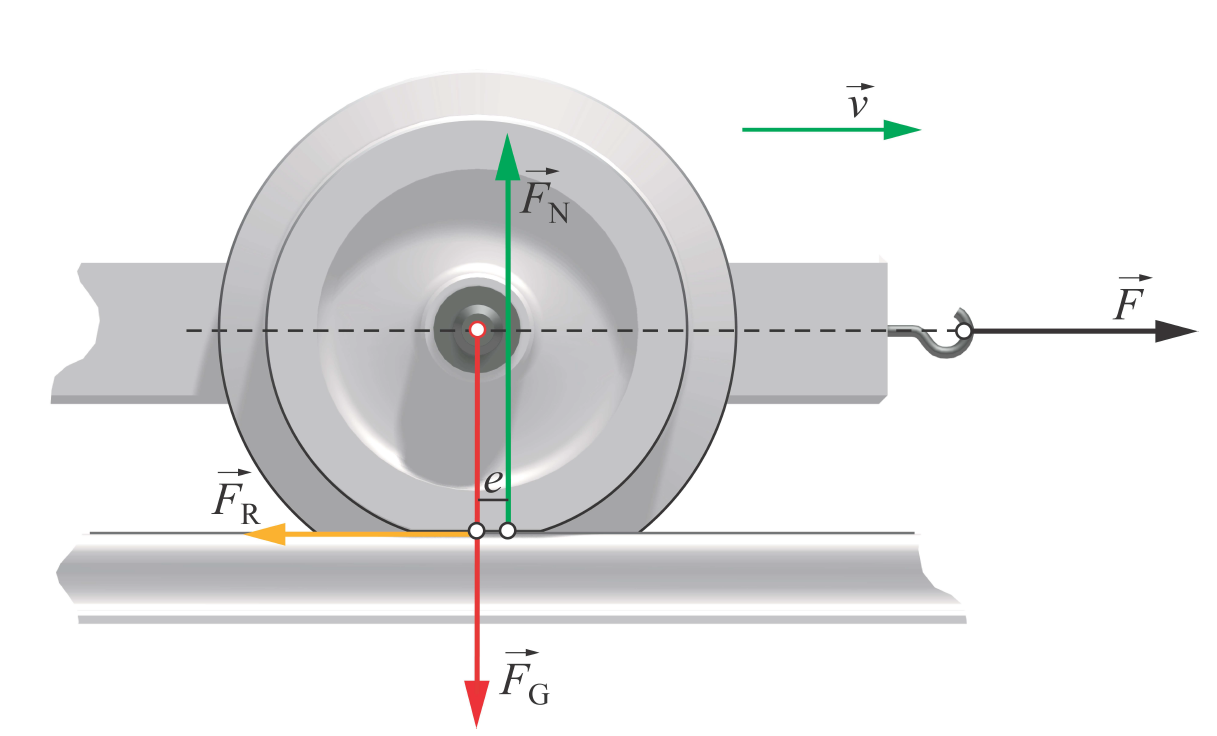
\includegraphics[width=0.8\linewidth]{Bilder/rollreibung_1} \\
		\end{minipage}
		\hfill
		\begin{minipage}{0.48\linewidth}
			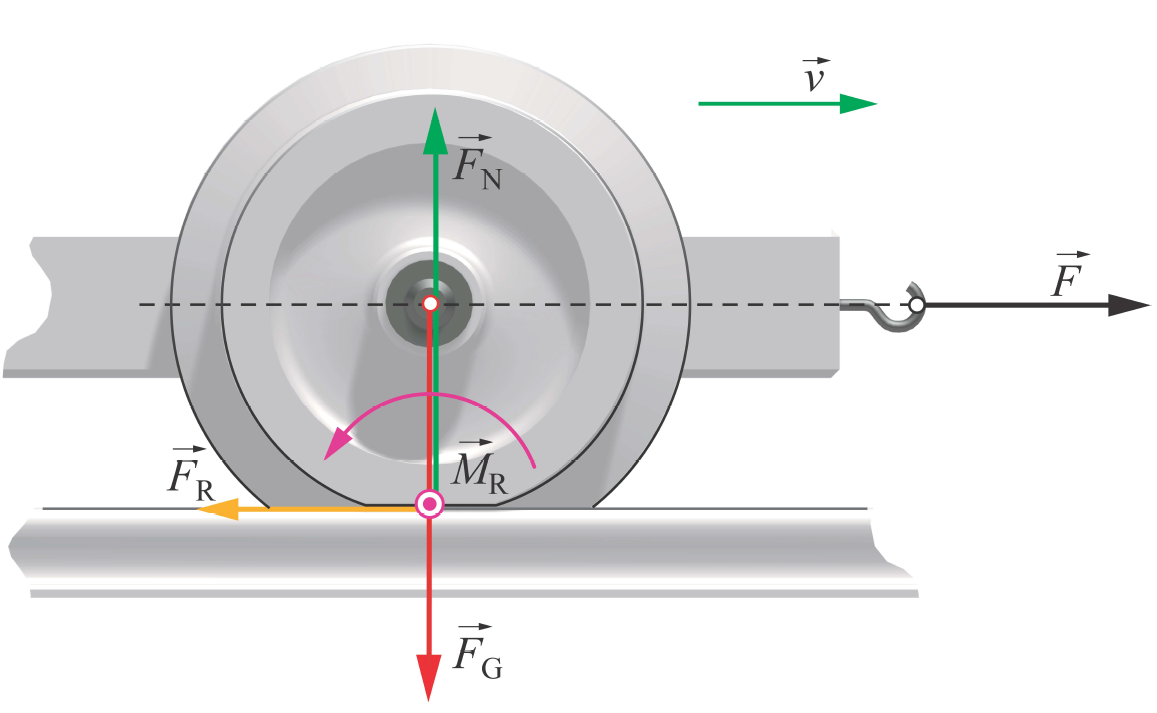
\includegraphics[width=0.8\linewidth]{Bilder/rollreibung_2} \\
		\end{minipage}
		
		$$ \boxed{ e = \frac{r \cdot F}{F_N} = \frac{r \cdot F_R}{F_N} =  \frac{r \cdot \mu_R \cdot F_R}{F_N} = \mu_R \cdot r }$$ 
		
		$$ \boxed{ M_R = e \cdot F_N = \mu_R \cdot r \cdot F_N = r \cdot F_R = r \cdot F} $$ \\

		\begin{tabular}{c l c}
			$e$ & Rollreibungslänge & $[e] = \mathrm{m}$ \\
			$r$ & Radius des Rades & $[r] = \mathrm{m}$ \\
			$F_R$ & Rollreibungskraft & $[F_R] = \mathrm{N}$ \\
			$F_N$ & Normalkraft & $[F_N] = \mathrm{N}$ \\
			$\mu_R$ & Rollreibungskoeffizient & $[\mu_R] = 1$ \\
			$M_R$ & Rollreibungsmoment & $[M_R] = \mathrm{Nm}$ \\
		\end{tabular}

	\subsection{Angetriebenes Rad}
	
		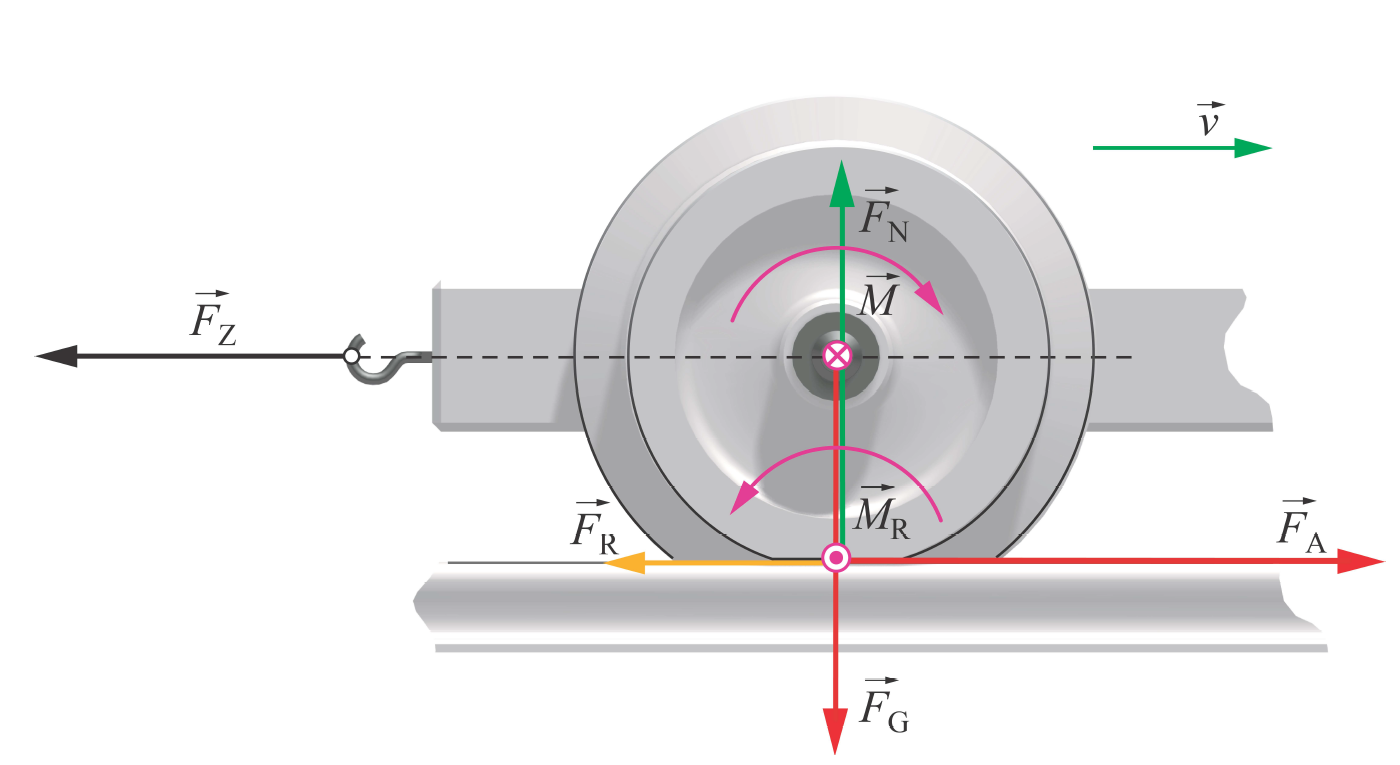
\includegraphics[width=0.8\linewidth]{Bilder/antriebsrad} \\
		\\

		\begin{tabular}{c l c}
			$\vec{F_Z}$ & Zugkraft & $[F_Z] = \mathrm{N}$ \\
			$\vec{F_N}$ & Normalkraft & $[F_N] = \mathrm{N}$ \\
			$\vec{F_R}$ & Rollreibungskraft & $[F_R] = \mathrm{N}$ \\
			$\vec{F_A}$ & Haftreibungskraft & $[F_A] = \mathrm{N}$ \\
		\end{tabular}

		\subsubsection{Hinweise zu Reibung an Rädern}
		
			\begin{tabular}{ll}
				$\bullet$ & Jedes Rad weist Rollreibung auf \\
				$\bullet$ & Zusätzlich zur Rollreibung weist ein angetriebenes Rad \\
				          & eine Haftreibung auf \\
			\end{tabular}

	\subsection{Arbeit und Energie}
	
		\subsubsection{Arbeit}
		
			Wird der Angriffspunkt einer Kraft $\vec{F}$ um die Strecke $d \vec{s}$ verschoben so leistet die Kraft die Arbeit $W$ 
			
			$$ \boxed{ W_{AB} =  \int \limits_A^B d \, W =  \int \limits_A^B \vec{F} \bullet d \, \vec{s} \qquad \text{(Skalarprodukt)} }$$ \\
			
			Wenn die projizierte Kraft konstant ist: $\boxed{ W = F \bullet s_{AB} }$ \\
			\\
			\begin{tabular}{c l c}
				$W$ & Arbeit & $[W] = \mathrm{N \cdot m = J}$ \\
				$F$ & Kraft & $[F] = \mathrm{N}$ \\
				$s$ & Weg & $[s] = \mathrm{m}$ \\
			\end{tabular}

		\subsubsection{Potentielle Energie $W_{pot}$}
			Beim Anheben eines Körpers gewinnt der Körper an potentieller Energie (Lageenergie) 
			
			$$ \boxed{ W_{pot} = m \cdot g \cdot h}$$
			\\
			\begin{tabular}{c l c}
				$W_{pot}$ & Potentielle Energie & $[W] = \mathrm{N \cdot m = J}$ \\
				$m$ & Masse des Körpers & $[m] = \mathrm{kg}$ \\
				$g$ & Erdbeschleunigung & $[g] = \mathrm{\frac{m}{s^2}}$ \\
				$h$ & Höhe der Körpers & $[h] = \mathrm{m}$ \\
				\\
			\end{tabular}
			
			\textbf{Beispiel: Spannen einer Feder} \\
				\\  
				Federkraft als Funktion der Auslenkung x \qquad $F = -k \cdot x$ \\
				\\
				$$ \boxed{ W_{pot} = \int \limits_0^{x_0}  - \vec{F} \bullet d \vec{x} = \int \limits_0^{x_0}  k \cdot x \, dx = \frac{1}{2} \, k \cdot \Delta x^2} $$ \\
				
			\begin{tabular}{c l c}
				$W_{pot}$ & Potentielle Energie & $[W] = \mathrm{N \cdot m = J}$ \\
				$F$ & Federkraft & $[F] = \mathrm{N} $ \\
				$k$ & Federkonstante & $[k] = \mathrm{\frac{N}{m}}$ \\
				$\Delta x$ & Auslenkung der Feder & $[\Delta x] = \mathrm{m}$ \\
			\end{tabular}

			\vfill\null
			\columnbreak

		\subsubsection{Kinetische Energie $W_{kin}$}
		
			$$ \boxed{ \normalsize{ W_{kin} = \int \limits_A^B \vec{F} \bullet d \, \vec{s} =  F \bullet s_{AB} = m \, a \cdot \frac{a}{2} t^2 = m \frac{a^2 \cdot t^2}{2} = \frac{1}{2} m \cdot v^2} }$$
			
			\begin{tabular}{c l c}
				$W_{kin}$ & Kinetische Energie & $[W] = \mathrm{N \cdot m = J}$ \\
				$F$ & Kraft & $[F] = \mathrm{N} $ \\
				$s$ & Wegstück (Kinematik) & $[s] = \mathrm{m}$ \\
				$m$ & Masse des Körpers & $[m] = \mathrm{kg}$ \\
				$a$ & Beschleunigung (Kinematik) & $[a] = \mathrm{\frac{m}{s^2}}$ \\
				$v$ & Geschwindigkeit (Kinematik) & $[v] = \mathrm{\frac{m}{s}}$ \\
			\end{tabular}

	\subsection{Energieerhaltung (in abgeschlossenen Systemen)}
	
		Die Gesamtenergie eines \underline{abgeschlossenen Systems} ist unveränderlich! \\
		\\
		\textbf{abgeschlossen: Es wird keine Masse hinzugefügt/entfernt und es wirken keine äusseren Kräfte!} \\
			\\	
			$$ \boxed{ W = \underbrace{m \cdot g \cdot h}_{\substack{\text{pot. Energie}}} =  m \cdot g \cdot \underbrace{ \frac{1}{2} \, g \cdot t^2}_{\substack{\text{h(t)}}}  = \underbrace{ \frac{1}{2} m \cdot v^2 }_{\substack{\text{kin. Energie}}} } $$ \\
			\\
			Für \underline{nicht abgeschlossene Systeme} kann eine Bilanzrechnung aufgestellt werden: \\
			Die Energiezunahme im Gesamtsystem entspricht der von aussen zugeführten Energie. \\
			Die Energieabnahme im Gesamtsystem entspricht der von aussen entzogenen Energie. \\

		\subsubsection{Energiesatz der Mechanik} 
			$$ \boxed{ E_{pot} + E_{kin} = E_{tot} = \text{const} } \qquad \text{(gilt zu jedem Zeitpunkt)} $$

	\subsection{Leistung und Wirkungsgrad}
	
		\subsubsection{Leistung}
		
			$$ \boxed{ P = \frac{\Delta W}{\Delta t} = \frac{\vec{F} \bullet \Delta \vec{s}}{\Delta t} = \vec{F} \frac{\Delta \vec{s}}{\Delta t} = \vec{F} \bullet \vec{v} } $$ 
			
			
			\begin{tabular}{c l c}
				$P$ & Leistung & $[P] = \mathrm{W = \frac{J}{s}}$ \\
				$\Delta W$ & geleistete Arbeit & $[W] = \mathrm{J}$ \\
				$\Delta t$ & verstrichene Zeit & $[t] = \mathrm{s}$ \\
				$F$ & Kraft & $[F] = \mathrm{N}$ \\
				$\Delta s$ & Wegstück & $[s] = \mathrm{m}$ \\
				\\
			\end{tabular}
			
			\textbf{Pferdestärken} \\
				\\
				$1 \; \mathrm{PS} = 75 \, \mathrm{kg} \cdot 9.81 \mathrm{\frac{m}{s^2}} \cdot 1 \mathrm{\frac{m}{s}} = 735.5 \, \mathrm{W}$ \\

		\subsubsection{Wirkungsgrad $\eta$}	
			Faustregel: Je grösser eine Maschine, desto besser ihr Wirkungsgrad \\
			
			$$ \boxed{ \eta = \frac{P_{ab}}{P_{zu}} } \qquad \textcolor{red}{\eta < 1} \qquad [\eta] = 1 $$

	\subsection{Impuls $\vec{p}$}
	
		$$ \boxed{ \vec{p} = m \cdot \vec{v} }$$ 
		
		2. Newton'sches Gesetz allgemeingültiger (relativistisch): \\
		
		$$ \boxed{ \vec{F} = m \cdot \vec{a} = m \cdot \frac{d \, \vec{v}}{dt} = \frac{d}{dt} (m \cdot \vec{v}) = \frac{d \, \vec{p}}{dt} } $$ 
		
		\begin{tabular}{c l c}
			$\vec{p}$ & Impuls & $[\vec{p}] = \mathrm{\frac{kg  \, m}{s}}$ \\
			$m$       & Masse & $[m] = \mathrm{kg}$ \\
			$\vec{v}$ & Geschwindigkeit & $[v] = \mathrm{\frac{m}{s}}$ \\
			$F$       & Kraft & $[F] = \mathrm{N}$ \\
			$\vec{a}$ & Beschleunigung & $[\vec{a}] = \mathrm{\frac{m}{s^2}}$ \\
		\end{tabular}

		\subsubsection{Kraftstoss $\Delta p$}
			Ein Kraftstoss entspricht einer Impulsänderung und kann über die mittlere Kraft beschrieben werden. \\
			\\
			\begin{minipage}{0.55\linewidth}
				$$ \boxed{ \int \limits_{t_a}^{t_a + \Delta t}  F(t) \, dt = \overline{F} \cdot \Delta t = \Delta p = p' - p } $$ 	
			\end{minipage}
			\hfill
			\begin{minipage}{0.42\linewidth}
				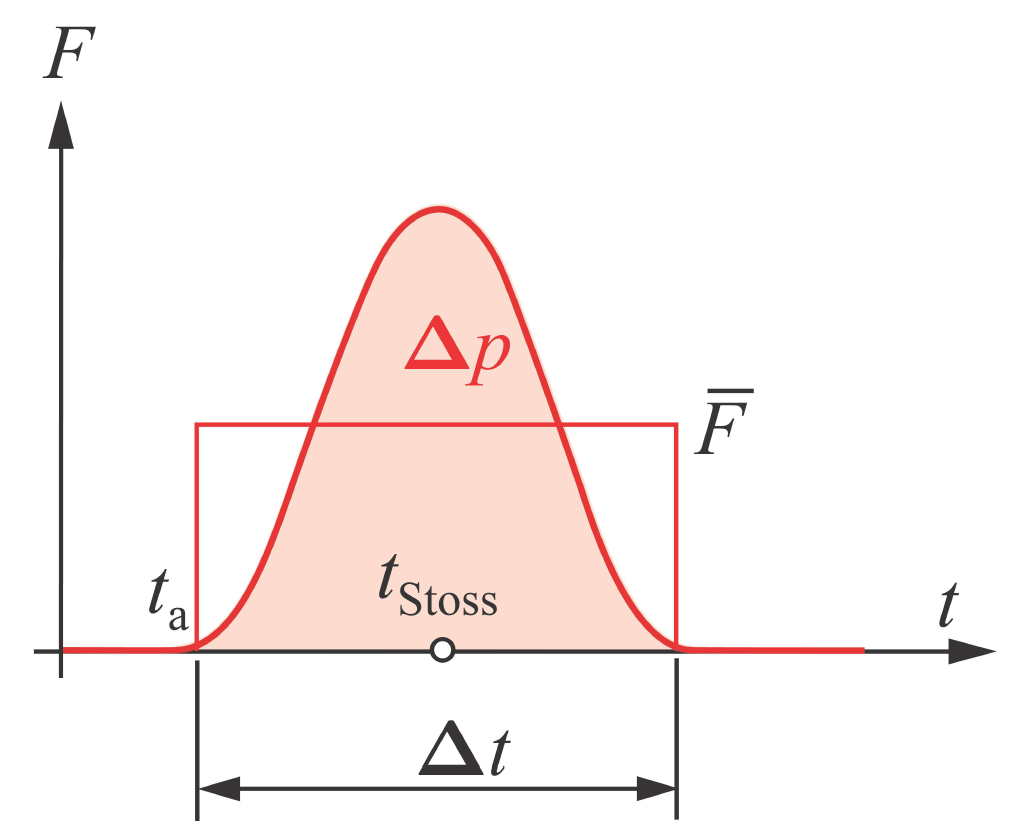
\includegraphics[width=0.8\linewidth]{Bilder/impuls} \\
			\end{minipage}
			
			\begin{tabular}{c l c}
				$F(t)$ & Kraftverlauf & $[F] = \mathrm{N}$ \\
				$\overline{F}$ & mittlere Kraft & $[\overline{F}] = \mathrm{N}$ \\
				$\Delta t$ & Zeitdauer des Kraftstosses & $[\Delta t] = \mathrm{s}$ \\
				$\Delta p$ & Impulsänderung & $[\Delta p] = \mathrm{Ns}$ \\
				$p$ & Impuls vor dem Stoss & $[p] = \mathrm{Ns}$ \\
				$p'$ & Impuls nach dem Stoss & $[p'] = \mathrm{Ns}$ \\
				$\vec{a}$ & Beschleunigung & $[\vec{a}] = \mathrm{\frac{m}{s^2}}$ \\
			\end{tabular}

	\subsection{Impulserhaltungssatz (Impulssatz)}
		In einem \textbf{abgschlossenen System} bleibt der Gesamtimpuls \\
		konstant \\
		abgeschlossenes System: es wirken keine externen Kräfte \\
		
		$$ \boxed{ \vec{p} =  \int \underbrace{  \frac{d \, \vec{p}}{dt} }_{\substack{F_{aussen} = 0}}   \, dt = c = \text{const} }  $$

	\subsection{Stösse}
	
		\begin{tabular}{ll}
			Elastizitätszahl: & $k = \frac{v_2' - v_1'}{v_1 - v_2} = - \frac{v'_{rel}}{v_{rel}} \geq 0$ \\
			\\
			Deformtionsarbeit: & $Q = (E_1 + E_2) - (E_1' + E_2') \geq 0$  \\
			\\
		\end{tabular}

		\begin{tikzpicture}
			[
			x=1cm, y=1cm, scale=0.5, font=\footnotesize, >=latex 
			%Voreinstellung für Pfeilspitzen
			]
			%Raster im Hintergrund
			%\draw[step=1, gray, very thin] (0,0) grid (5.5,5.5);
			
			%m1
			\begin{scope}[xshift=0cm, yshift=0cm, rotate=0, scale=1]
				%Kräfte
				\fill[gray!50!white] (0, 0) circle(1.25);
				\draw[thick] (0, 0) circle(1.25);
				\fill[black] (0, 0) circle(5pt) node [midway, above, yshift=2pt, scale=1.5] {$m_1$};
				\draw [-latex, very thick, purple] (1.25,0) -- ++(1.5,0) node[midway, above, scale=1.5] {$\vec{v}_1$};
			\end{scope}		
			
			%m2
			\begin{scope}[xshift=4cm, yshift=0cm, rotate=0, scale=1]
				%Kräfte
				\fill[gray!50!white] (0, 0) circle(0.75);
				\draw[thick] (0, 0) circle(0.75);
				\fill[black] (0, 0) circle(5pt) node [midway, above, yshift=2pt, scale=1.5] {$m_2$};
				\draw [-latex, very thick, purple] (0.75,0) -- ++(1.5,0) node[midway, above, scale=1.5] {$\vec{v}_2$};
			\end{scope}	
		\end{tikzpicture}

		\subsubsection{Gerader, zentraler, total elastischer Stoss}
			Die beiden Stosspartner verformen sich nicht!\\
			$\Rightarrow$ Für die Deformationsarbeit gilt: $Q = 0$ \\
			\boxed{
				\begin{tabular}{ll}
					Impulssatz: &  $p  \overset{!}{=} p'$ \\
					& $m_1 \, v_1 + m_2 \, v_2 \overset{!}{=} m_1 \, v_1' + m_2 \, v_2'$ \\
					\\
					Energiesatz: & $E_{kin} \overset{!}{=} E_{kin}'$ \\
					& $\frac{1}{2} m_1 \, v_1^2 + \frac{1}{2} m_2 \, v_2^2 \overset{!}{=} \frac{1}{2} m_1 \, v_1'^2 + \frac{1}{2} m_2 \, v_2'^2 $ \\
					\\
					& $v_1' = \frac{m_1 - m_2}{m_1 + m_2} \cdot v_1 + \frac{2 \, m}{m_1 + m_2} \cdot v_2$ \\
					\\
					& $v_2' = \frac{2 \, m_1}{m_1 + m_2} \cdot v_1 + \frac{m_2 - m_1}{m_1 + m_2} \cdot v_2$ \\
				\end{tabular}
			}

		\subsubsection{Gerader, zentraler, total inelastischer Stoss}
			Die beiden Stosspartner haften nach dem Stoss aneinander und haben die gleiche Geschwindigkeit. \\
			$\Rightarrow$ Für die Deformationsarbeit gilt: $Q \neq 0$ \\
			\boxed{
				\begin{tabular}{ll}
					Impulssatz: & $p  \overset{!}{=} p'$ \\
					& $m_1 \, v_1 + m_2 \, v_2 \overset{!}{=} (m_1 + m_2) \, v'$ \\
					\\
					Energiesatz: & $E_{kin} \overset{!}{=} E_{kin}'$ \\
					& $\frac{1}{2} m_1 \, v_1^2 + \frac{1}{2} m_2 \, v_2^2 \overset{!}{=} \frac{1}{2} (m_1 + m_2) \, v'^2 + Q$ \\
					\\
					Deformationsarbeit: & $Q = \frac{m_1 \, m_2}{2 (m_1 + m_2)} (v_1 - v_2)^2 =  \frac{1}{2} \mu \cdot v_{rel}^2 $ \\
					\\
					Relativgeschw.: & $v_{rel} := \vert v_1 - v_2  \vert$ \\
					\\
					Reduzierte Masse: & $\mu = \frac{m_1 \, m_2}{m_1 + m_2}$\\
				\end{tabular}
			}

			\begin{tabular}{c l c}
				$k$ & Elastizitätszahl & $[k] = 1$ \\
				$E_1, \,E_2$ & Energien vor Stoss & $[E] = \mathrm{J}$ \\	
				$E_1 ', \, E_2 '$ & Energien nach Stoss & $[E'] = \mathrm{J}$ \\	
				$m_1, \, m_2$ & stossende Massen & $[m] = \mathrm{kg}$ \\
				$v_1, \, v_2$ & Geschwindigkeit vor Stoss & $[v] = \mathrm{\frac{m}{s}}$ \\
				$v_1', \, v_2'$ & Geschwindigkeit nach Stoss & $[v'] = \mathrm{\frac{m}{s}}$ \\
				$Q$ & Deformationsarbeit & $[Q] = \mathrm{J}$ \\
				$v_{rel}$ & Relativgeschwindigkeit &  $[v_{rel}] = \mathrm{\frac{m}{s}}$ \\
				$\mu$ & reduzierte Masse & $[\mu] = \mathrm{kg}$ \\
			\end{tabular}

	\subsection{Rakete}
		\subsubsection{Rakete im Flug}
			$\Rightarrow$ Masse ist hier veränderbar! \qquad $m(t) = m = m_{Start} - \mu \cdot t$ \\
			\\
			Die Rakete verliert an Treibstoff, wodurch die Masse der Rakete abnimmt ($dm < 0$)\\
			\\	
			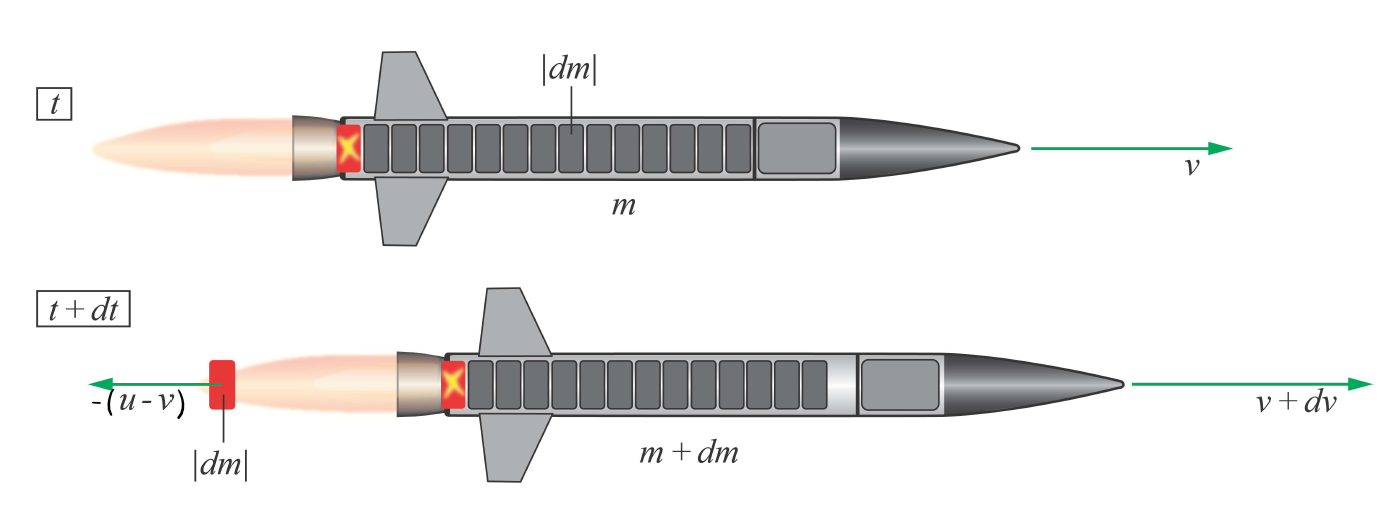
\includegraphics[width=0.73\linewidth]{Bilder/rakete} \\
			\\
			Impulssatz: \quad $ m \cdot v(t) = (m + dm)(v(t) + dv) + dm \,(u-v) $ \qquad $dm < 0$ \\
			\\
			Raketengleichung: $v(t) = - u \cdot \ln(m) + v_0 + u \cdot \ln(m_0) = v_0 + u \cdot \ln(\frac{m_0}{m})$ \\
			\\
			Massenverhältnis: $\frac{Startmasse}{Endmasse}$ \\
			\\
			max. Geschwindigkeitsänderung: $\Delta v = v - v_0 = u \cdot \ln(\frac{m_0}{m})$ \\
			\\
			Schubkraft: $F_{Schub} = \frac{dp}{dt} = - \frac{u \cdot dm}{dt} =  \underbrace{ \frac{dm}{dt} }_{\substack{\mu}} (-u) = \mu \cdot u$ \\ 
			\\
			$\Rightarrow$ Hier wurde noch keine Erdbeschleunigung (Anziehung) berücksichtigt! \\
			\\
			\\
			\begin{tabular}{c l c}
				$u$ &  Strahlgeschwindigkeit der Rakete & $[u] =  \mathrm{\frac{m}{s}}$ \\	
				$m$ & Zeitlich veränderbare Masse $m(t)$ & $[m] = \mathrm{kg}$ \\
				$m_0$ & Masse zum Startzeitpunkt & $[m] = \mathrm{kg}$ \\
				$v_0$ & Startgeschwindigkeit & $[v_0] = \mathrm{\frac{m}{s}}$ \\
				$F_{Schub}$ & Schubkraft der Rakete & $[F_{Schub}] = \mathrm{N}$ \\
				$\mu$ & Treibstoffverbrauch pro Zeit & $[\mu] = \mathrm{\frac{kg}{s}}$
			\end{tabular}

		\subsubsection{Aufstieg der Rakete im Schwerefeld}
			Konstante Erdbeschleunigung g wird berücksichtigt \\
			\\
			Veränderbare Masse: $m(t) = m = m_{Start} - \mu \cdot t$ \\
			\\
			Gesamtkraft: $m(t) \frac{dv}{dt} = m(t) \cdot a = F_{Schub} - F_G = \mu \cdot u - m \cdot g$ \\
			\\
			Beschleunigung: $a(t) = \frac{dv}{dt} = \frac{\mu \cdot u}{m_0 - \mu \cdot t} - g$ \\
			\\
			Raketengleichung: $v(t) = u \cdot \ln( \frac{m_{Start}}{m(t)} ) -  g \cdot t  $ \\
			\\
			Spezifischer Impuls: $T = \frac{m(t)}{\mu} = \frac{u}{g}$ \\
			\\
			Steighöhe: $h_t = u \cdot t - \frac{1}{2}gt^2 - \frac{u}{\mu} \cdot ln(\frac{m_0}{m_t}) \cdot m_t $
			\\
			\begin{tabular}{c l c}
				$u$ &  Strahlgeschwindigkeit der Rakete & $[u] =  \mathrm{\frac{m}{s}}$ \\	
				$m$ & Zeitlich veränderbare Masse $m(t)$ & $[m] = \mathrm{kg}$ \\
				$m_0$ & Masse zum Startzeitpunkt & $[m] = \mathrm{kg}$ \\
				$v_0$ & Startgeschwindigkeit & $[v_0] = \mathrm{\frac{m}{s}}$ \\
				$g$ & Erdbeschleuigung & $[g] = \mathrm{\frac{m}{s^2}}$ \\
				$\mu$ & Treibstoffverbrauch pro Zeit & $[\mu] = \mathrm{\frac{kg}{s}}$ \\
				$T$ & spezifischer Impuls (Zeit von konstantem Schub) & $[T] = \mathrm{s}$  \\
			\end{tabular}

	\subsection{Gravitation}
		\subsubsection{Erstes Kepler'sches Gesetz}
			Die Planeten bewegen sich auf Ellipsen, in deren Brennpunkt sich die Sonne befindet. \\
			\\
			\begin{minipage}{0.45\linewidth}
				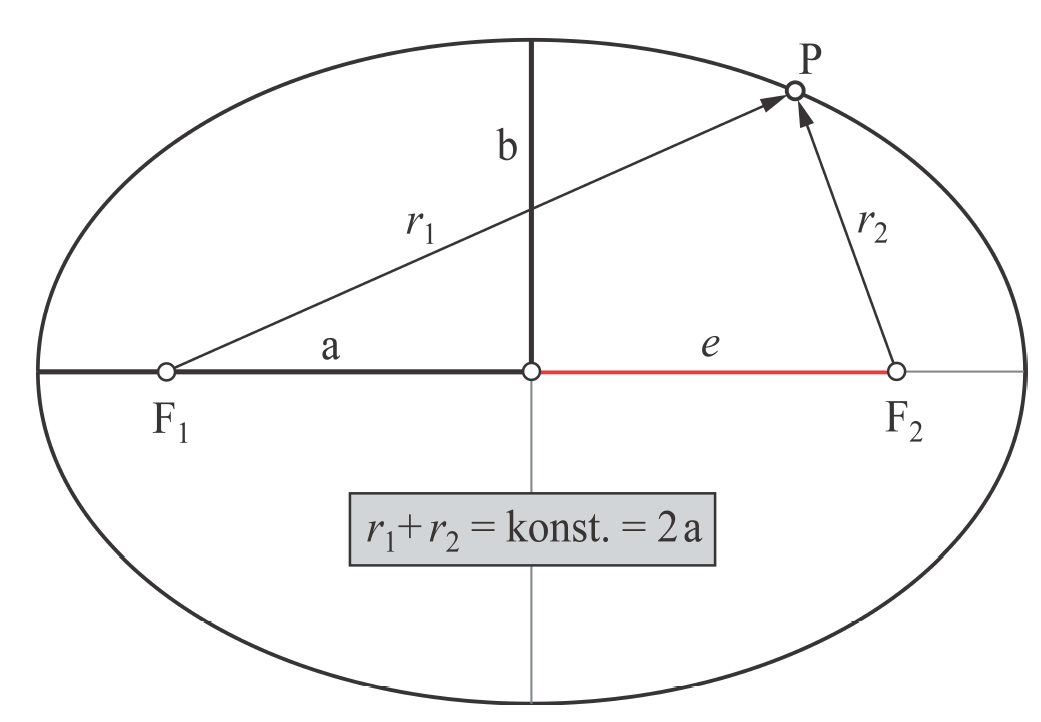
\includegraphics[width=\linewidth]{Bilder/ellipse}
			\end{minipage}
			\hfill
			\begin{minipage}{0.53\linewidth}
				\begin{tabular}{ll}
					$a$ & grosse Halbachse \\
					$b$ & kleine Halbachse \\
					$F_1, F_2$ & Brennpunkte \\
					$e$ & Exzentrizität \\
					$\epsilon$ & num. Exzentrizität $\epsilon = \frac{e}{a} $\\	
					$r_{min}$ & minimaler Radius \\	
					& $r_{min} = a \,(1 - \epsilon)$ \\
					$r_{max}$ & maximaler Radius \\
					& $r_{max} = a \,(1 + \epsilon)$ \\
				\end{tabular}
			\end{minipage}

		\subsubsection{Zweites Kepler'sches Gesetz}
			Der Fahrstrahl der Planeten überstreicht in der gleichen Zeit die gleiche Fläche. \\
			$\Rightarrow$ Bei kleinerem Abstand zur Sonne ist die Geschwindigeit schneller! \\
		
		\subsubsection{Drittes Kepler'sches Gesetz}
			Die Quadrate der Umlaufzeiten verhalten sich wie die Kuben der grossen Halbachsen. \\
			\\
			$a = \big(  \frac{T}{T_{ref}}^{\frac{2}{3}} \cdot a_{ref} \big)$ \qquad $\Leftrightarrow$ \qquad $\big( \frac{a}{a_{ref}}  \big)^3 =  \big( \frac{T}{T_ref}  \big)^2 $ \\
			\\
			Als Referenz wird die Erde verwendet! \\
			\\
			Astronomische Einheit: $a_{ref} = 1 \, \mathrm{AE} = 149.6 \cdot 10^6 \, \mathrm{km}$ \\
			\\
			Referenzzeit: $T_{ref} = 1 \, a = 1 \; \mathrm{Jahr}$ \\
			\\
			\begin{tabular}{c l c}
				$a$ & grosse Halbachse gesuchtet Planet & $[a] = \mathrm{AE}$ \\
				$a_{ref}$ &  grosse Halbachse Erde & $[a_{ref}] = \mathrm{AE}$ \\	
				$T$ & Umlaufzeit Planet & $[T] = \mathrm{Jahre}$ \\
				$T_{ref}$ & Umlaufzeit Erde & $[T] = \mathrm{Jahre}$ \\
			\end{tabular}

		\subsubsection{Gravitationsgesetz}
		
			$$ \boxed{ \text{Gravitationskraft:}  \quad F_G = G \, \frac{m_1 \cdot m_2}{r^2} \quad \text{mit }G = 6.67 \cdot 10^{-11} \mathrm{\frac{m^3}{kg \, s^2}} }$$ 

		\subsubsection{Gravitationswirkung innerhalb einer Kugel}
		
			$$ \boxed{ F_G = G \, \frac{m_{Kern} (r) \, m}{r^2} =  G \, \frac{4 \, \pi \, r^3 \, \rho \, m}{3 \, r^2} = \frac{4 \, \pi}{3} \, G \, \rho \, m \, r } $$ \\
		
			\begin{tabular}{c l c}
				$F_G$ & Gravitationskraft & $[F_G] = \mathrm{N}$ \\
				$G$ & Gravitationskonstante & $[G] = \mathrm{\frac{m^3}{kg \, s^2}}$ \\	
				$r$ & Radius (Abstand vom Zentrum) & $[r] = \mathrm{m}$ \\
				$\rho$ & homogene Dichte der Kugel & $[\rho] = \mathrm{\frac{kg}{m^3}}$ \\
				$m$ & Masse vom Massepunkt & $[m] = \mathrm{kg}$ \\
				$m_{Kern}$ & Masse des Kugelkerns & $[m_{Kern}] = \mathrm{kg}$ \\
			\end{tabular}

		\subsubsection{Gravitationswirkung ausserhalb einer Kugel}
		
			$$ \boxed{ F_G = G \, \frac{M \cdot m}{r^2}}  $$ \\
			
			\begin{tabular}{c l c}
				$F_G$ & Gravitationskraft & $[F_G] = \mathrm{N}$ \\
				$G$ & Gravitationskonstante & $[G] = \mathrm{\frac{m^3}{kg \, s^2}}$ \\	
				$r$ & Radius (Abstand vom Zentrum) & $[r] = \mathrm{m}$ \\
				$m$ & Masse vom Massepunkt & $[m] = \mathrm{kg}$ \\
				$M$ & Gesamtmasse der Kugel & $[M] = \mathrm{kg}$ \\
			\end{tabular}

		\subsubsection{Gravitationspotential  $\phi$}
		
			Wenn eine Masse in einem Gravitationsfeld bewegt wird, so wird Arbeit verrrichtet. \\
			\\
			$$ \boxed{ W_{12} = \int \limits_{r_1}^{r_2} \vec{F}_G \bullet d \vec{s}  =  \int \limits_{r_1}^{r_2} G \, \frac{M \cdot m}{r^2} \, dr = G \cdot M \cdot m \big( \frac{1}{r_2} - \frac{1}{r_1}  \big) }  $$  
			
			$$ \boxed{ \text{potentielle Energie:} \quad E_{pot}(r) = -G \, \frac{M \, m}{r} }$$ 
			
			$$ \boxed{ \text{Gravitationspotential:} \quad \phi = \frac{E_{pot}}{m} = - \frac{G \cdot M}{r}}  $$ \\

			\textbf{Im Inneren eines homogenen Zentralkörpers gilt} \\
			
				$$ \boxed{ F_G = \frac{4 \, \pi \cdot G \cdot \rho \cdot m \cdot r}{3} }$$ 
				
				$$ \boxed{ E_{pot} = - \frac{2 \,  \pi \cdot G \cdot \rho \cdot m}{3} \, r^2 + c' } $$
				
				$$ \boxed{ \phi = - \frac{2 \,  \pi \cdot G \cdot \rho}{3} \, r^2 + c = - \frac{G \cdot M(r)}{2 \, r}  + c = - \frac{G \cdot M(r)}{2 \, r} - \frac{G \cdot M}{2 \, R} } $$ \\
				
			\begin{tabular}{c l c}
				$W$ & Arbeit & $[W] = \mathrm{J} $ \\
				$F_G$ & Gravitationskraft & $[F_G] = \mathrm{N}$ \\
				$E_{pot}$ & potentielle Energie & $E_{pot} = \mathrm{J}$ \\
				$G$ & Gravitationskonstante & $[G] = \mathrm{\frac{m^3}{kg \, s^2}}$ \\	
				$r$ & Radius (Abstand vom Zentrum) & $[r] = \mathrm{m}$ \\
				$\rho$ & homogene Dichte der Kugel & $[\rho] = \mathrm{\frac{kg}{m^3}}$ \\
				$m$ & Masse vom Massepunnkt & $[m] = \mathrm{kg}$ \\
				$M$ & Gesamtmasse der Kugel & $[M] = \mathrm{kg}$ \\
				$R$ & Radius der Kugeloberfläche & $[R] = \mathrm{m}$ \\
			\end{tabular}

	\subsection{Bezugssysteme: Inertialsystem}
		Inertialsystem: \textbf{unbeschleuigtes} Bezugssystem \\
		\\
		Wenn die Newton'schen Gesetze im Bezugssystem S gelten, so gelten sie auch im Bezugssystem S', solange dieses nicht beschleunigt ist und nicht rotiert. \\
		$\Rightarrow$ \textbf{In sämtlichen Inertialsystemen sind die mechanischen Gesetze identisch!} \\

		\subsubsection{Galilei-Transformation}
			\begin{minipage}{0.48\linewidth}
				Bezugssystem S' bewegt sich mit konstanter Geschwindigkeit $v_0$: \\
				\\
				\\
				$v_0 = \begin{pmatrix}v_x \\ v_y \\ v_z\end{pmatrix}$
			\end{minipage}
			\hfill
			\begin{minipage}{0.42\linewidth}
				Transformation zwischen \\
				S und S' \\
				\\
				$x = x' + v_x t$ \\
				$y = y' + v_y t$ \\
				$z  = z' + v_z t$ \\
				$t = t'$
			\end{minipage}

	\subsection{Beschleunigte Bezugssysteme}
		In beschleunigten Bezugssystemen müssen \textbf{Trägheitskräfte} berücksichtigt werden!

		\subsubsection{Translatorisch beschleunigtes Bezugssystem}
			Beispiel: Zug beschleunigt auf gerader Schiene \\
			\\
			Für einen Beobachter \textbf{im beschleunigten System} S' wirkt \\
			eine Trägheitskraft: 
			
			$$ \boxed{ \text{Gesamtkraft:} \quad \vec{F}' = \vec{F} - m \cdot \vec{a}_0 = \vec{F} + \vec{F}_{Tr"agheit} }$$ \\
			
			\begin{tabular}{c l c}
				$\vec{F}'$ & Gesamte im System wirkende Kraft & $[\vec{F}'] = \mathrm{N}$ \\
				$\vec{F}$ & Statisch wirkende Kräfte & $[\vec{F}] = \mathrm{N}$ \\
				$\vec{F}_{Tr"agheit}$ & Trägheitskraft & $[\vec{F}_{Tr"agheit}] = \mathrm{N}$ \\
				$m$ & Masse im System & $[m] = \mathrm{kg}$ \\
				$\vec{a}_0$ & Beschleunigung des Systems & $[\vec{a}_0] = \mathrm{\frac{m}{s^2}}$ \\
			\end{tabular}

		\subsubsection{Gleichförmig rotierendes Bezugssystem (Scheinkräfte)}

			\textbf{Fest verbundene Masse} $\Rightarrow$ \textbf{Scheinkraft: Zentrifugalkraft} \\
				\\
				\begin{minipage}{0.48\linewidth}
					$$ \boxed{ \vec{F}_z = - m \, \vec{a}_z = - m \cdot \omega^2 \cdot \vec{r} }$$ 
					
					$$ \boxed{ \vec{F}_{Zentrifugal}  \overset{!}{=} - \vec{F}_{Zentripetal} }$$ 
				\end{minipage}
				\hfill
				\begin{minipage}{0.48\linewidth}
					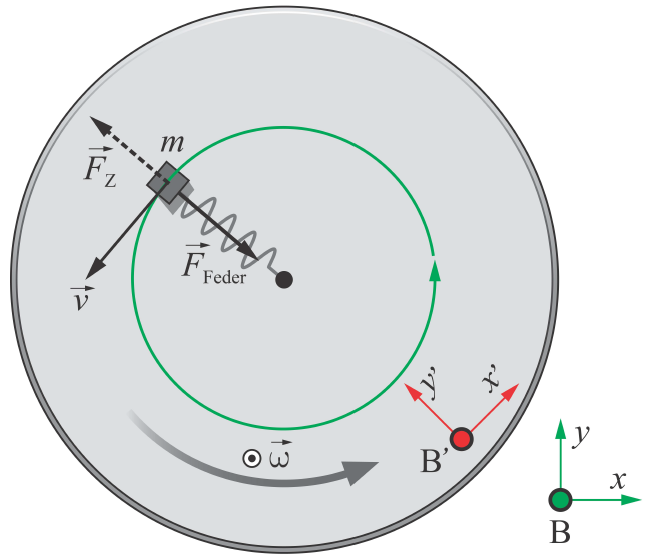
\includegraphics[width=0.75\linewidth]{Bilder/zentrifugalkraft} \\
				\end{minipage}
				\\
				\begin{tabular}{c l c}
					$\vec{F}_z$ & Zentrifugalkraft (Trägheitskraft; Scheinkraft) & $[\vec{F}_z] = \mathrm{N}$ \\
					$m$ & Masse im System & $[m] = \mathrm{kg}$ \\
					$\vec{a}_z$ & Beschleunigung des Systems ($a_{radial}$) & $[\vec{a}_z] = \mathrm{\frac{m}{s^2}}$ \\
					$\omega$ & Winkelgeschwindigkeit & $[\omega] = \mathrm{\frac{rad}{s}}$ \\
					$\vec{r}$ & Radius des Systems (nach innen zeigend) & $[\vec{r}] = \mathrm{m}$ \\ 
					\\
					\\
				\end{tabular}

			\textbf{lose Masse} $\Rightarrow$ \textbf{Scheinkraft: Corioliskraft} \\	
				\\
				\\
				\begin{minipage}{0.48\linewidth}
					$$ \boxed{\vec{F}_c = - m \cdot \vec{a}_c = - m \cdot 2 \, (\vec{\omega} \times \vec{v}_R)} $$ 
				\end{minipage}
				\hfill
				\begin{minipage}{0.48\linewidth}
					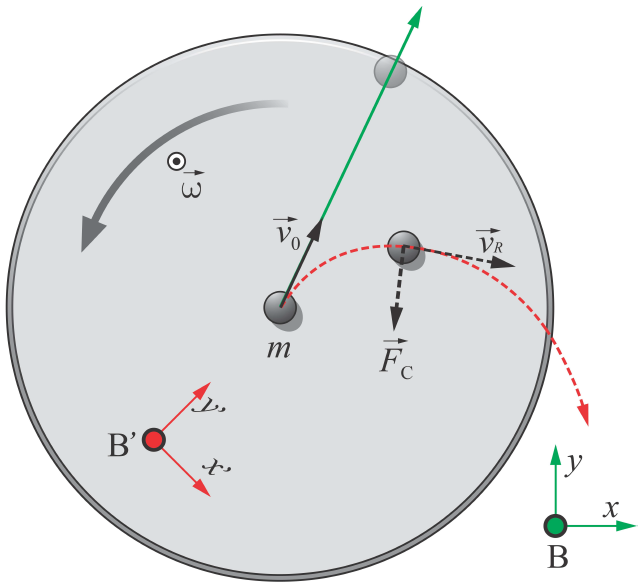
\includegraphics[width=0.75\linewidth]{Bilder/corioliskraft} \\
				\end{minipage}
				\\
				\begin{tabular}{c l c}
					$\vec{F}_c$ & Corioliskraft (Trägheitskraft; Scheinkraft) & $[\vec{F}_c] = \mathrm{N}$ \\
					$m$ & Masse im System & $[m] = \mathrm{kg}$ \\
					$\vec{a}_c$ & Coriolisbeschleunigung & $[\vec{a}_c] = \mathrm{\frac{m}{s^2}}$ \\
					$\omega$ & Winkelgeschwindigkeit & $[\omega] = \mathrm{\frac{rad}{s}}$ \\
					$\vec{v}_R$ & Relativgeschwindigkeit & $[\vec{v}_R] = \mathrm{\frac{m}{s}}$ \\ 
				\end{tabular}

		\subsubsection{D'Alembert'sches Prinzip}
			Wird ein Körper in einem mitbewegten Koordinatensystem \\
			betrachtet, so bleibt er in Ruhe: \quad $\vec{v}_R = 0$ und $\vec{a}_R = 0$ \\
			
			$$ \boxed{ \vec{F} + \underbrace{ \vec{F}_z + \vec{F}_c }_{\substack{\text{Scheinkräfte}}} = \vec{0} }$$ 
			
			$\Rightarrow$ Statisches Gleichgewichtsproblem

	\subsection{Rotation starrer Körper}
	
		\begin{tabular}{ll}
			Rotation: & Drehung um feste Achse \\
			Kreisel: & Drehung um starren Punkt \\
			Kreiselbewegung & Drehung eines völlig freien, \\
			&  starren Körpers um seinen Schwerpunkt \\
		\end{tabular}

		\subsubsection{Dynamisches Grundgesetz der Rotation}
			Es ist \textbf{nur die tangentiale Komponente} der Kraft \\
			(des Drehmoments) eines rotierenden Körpers relevant! \\
				
			$$dM_t = r \cdot dF_t = r \cdot dm \cdot a_t = dm \cdot r^2 \cdot \alpha$$ \\
			
			$$ \boxed{ M = \int dM = \int r^2 \, \alpha \cdot dm = \alpha  \underbrace{  \int r^2 \cdot dm }_{\substack{J_{Scheibe} = m \cdot r^2}} }$$ \
			
			$$ \boxed{ \Rightarrow \; M = J \cdot \alpha = r \cdot F} $$ \\
				
			\begin{tabular}{c l c}
				$dM_t$ & kleine Tan.-Komponente des Drehmoments & $[dM_t] = \mathrm{Nm}$ \\
				$M$ & (gesamtes) Drehmoment & $[M] = \mathrm{Nm}$ \\
				$dF_t$ & kleine Tangentialkomponente der Kraft & $[dF_t] = \mathrm{N}$ \\
				$r$ & Abstand Drehachse zu Massepunkt (Rand) & $[r] = \mathrm{m}$ \\
				$dm$ & kleines Massestück des Körpers & $dm = \mathrm{kg}$ \\
				$a_t$ & Tangentialbeschleunigung ($a_t = r \cdot \alpha$) & $[a_t] = \mathrm{\frac{m}{s^2}}$ \\
				$\alpha$ & Winkelbescheunigung & $[\alpha] = \mathrm{\frac{rad}{s^2}}$ \\
				$J$ & (Massen-) Trägheitsmoment & $[J] = \mathrm{kg \, m^2}$ \\
			\end{tabular}

		\subsubsection{Massenträgheitsmomente} %TODO: Irgendwann mal Bilder gegen ganze Tabelle tauschen
		
			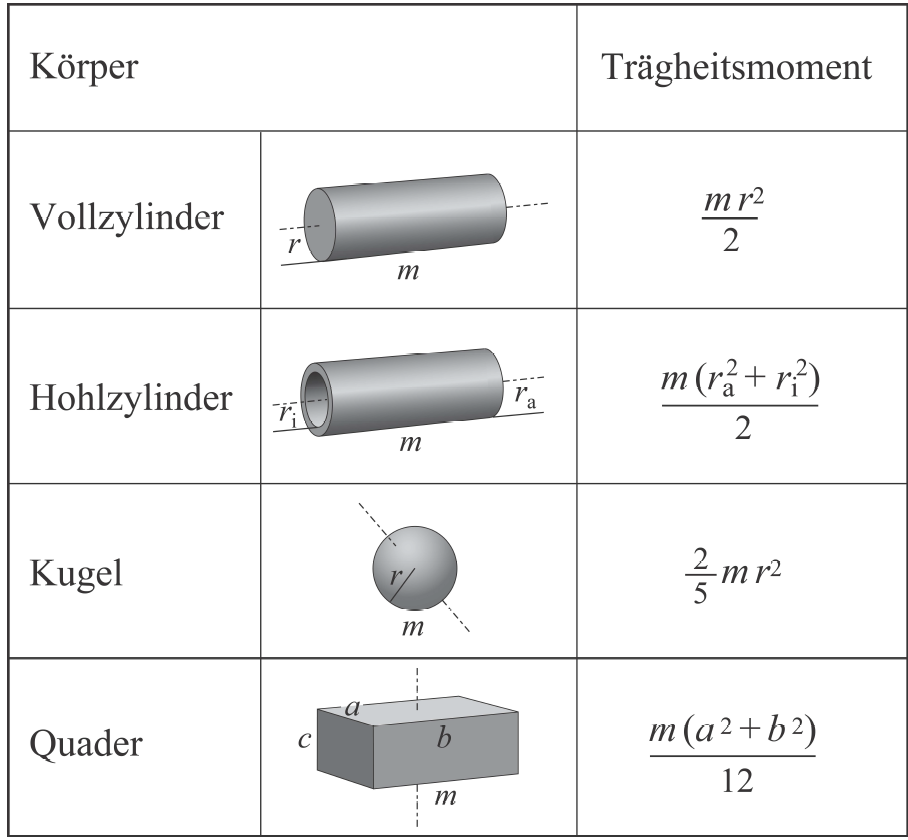
\includegraphics[width=0.8\linewidth]{Bilder/massentraegheitsmomente}

			Ring: $m \cdot r^2$

	\subsection{Trägheitsellipsoid}
		Trägheitsradius $r_0$: als ob ganze Masse eines Körpers nur einen \\
		Radius hätte \\
		\\
		\begin{minipage}{0.48\linewidth}
			$$ \boxed{ r_0 = \sqrt{\frac{J}{m}}} $$
		\end{minipage}
		\hfill
		\begin{minipage}{0.48\linewidth}
			$$ \boxed{s_0 = \frac{1}{r_0} }$$
		\end{minipage}
		
		\begin{tabular}{c l c}
			$r_0$ & Trägheitsradius & $[r_0] = \mathrm{m}$ \\
			$m$ & Masse des Körpers & $[m] = \mathrm{kg}$ \\
			$J$ & (Massen-) Trägheitsmoment & $[J] = \mathrm{kg \, m^2}$ \\
			$s_0$ & reziproker Trägheitsradius & $[s_0] = \mathrm{m}$ \\
			\\
		\end{tabular}
		
		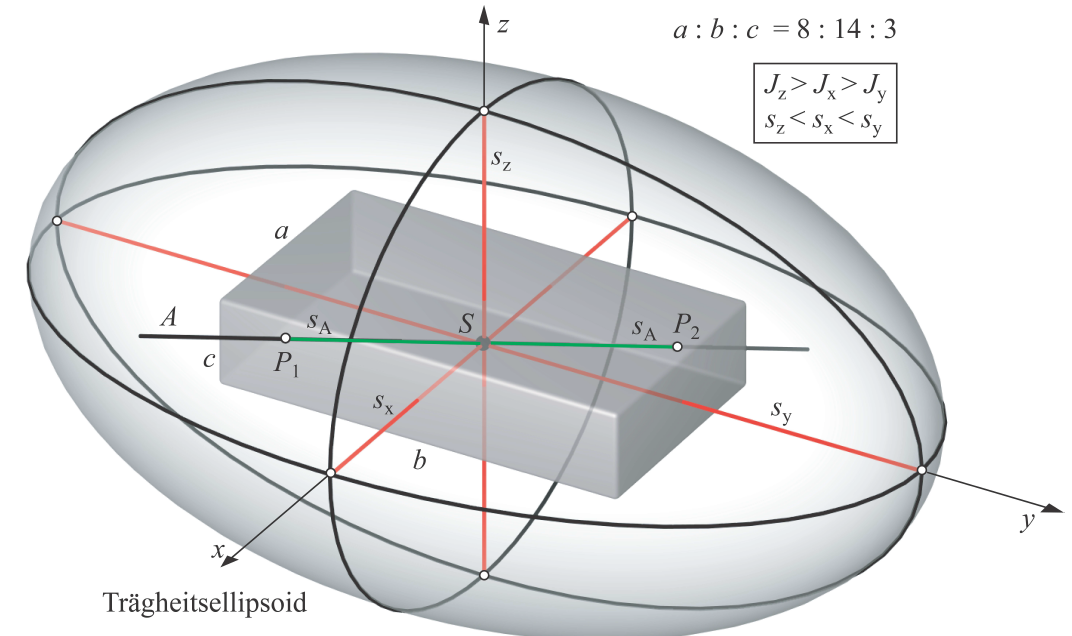
\includegraphics[width=0.8\linewidth]{Bilder/traegheits_ellipsoid} \\	
		\\
		\textcolor{red}{Hauptträgheits-Achsen} (entsprechen immer Symmetrie-Achsen, falls vorhanden) \\
		\textcolor{green}{beliebige Achse $J_A$} \quad $J_A = J_x \cdot \cos^2(\alpha) + J_y \cdot \cos^2(\beta) + J_z \cdot \cos^2(\gamma)$

	\subsection{Satz von Steiner}
		Beschreibt, wie man das Trägheitsmoment $J$ berechnet, wenn die Drehachse nicht durch den Schwerpunkt des rotierenden Körpers geht, sonden \textbf{parallel} dazu verläuft. \\
		
		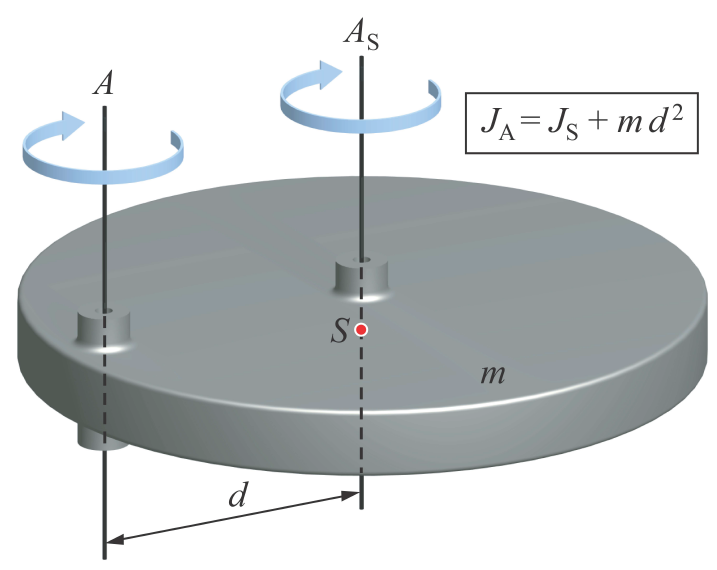
\includegraphics[width=0.6\linewidth]{Bilder/steiner} \\	
		\\
		\begin{tabular}{c l c}
			$J_S$ & Trägheitsmoment (Rot. um Schwerp.)  & $[J_S] = \mathrm{kg \, m^2}$ \\
			$J_A$ & Trägheitsmoment (Rot. um bel. Punkt)  & $[J_A] = \mathrm{kg \, m^2}$ \\
			$m$ & Masse des Körpers & $[m] = \mathrm{kg}$ \\
			$d$ & Abstand zum Schwerpunkt & $[d] = \mathrm{m}$ \\
		\end{tabular}

	\subsection{Arbeit und Leistung (Rotation)}
		$dW = \vec{F} \bullet d\vec{s} = F_t \cdot ds = F_t \cdot r \cdot d \phi = M \cdot d \phi $ \\
		\\
		$P = \frac{dW}{dt} = M \frac{d \phi}{dt} = M \cdot \omega$ \\
		\\
		\begin{tabular}{c l c}
			$F_t$ & \textbf{Tantentialer} Kraftanteil der Rotation & $[F_t] = N$ \\
			$d \phi$ & zurückgelegter Kreiswinkel & $[d \phi] = rad$ \\	
			$P$ & Leistung  & $[P] = W$ \\
			$W$ & Energie  & $[W] = J$ \\
			$\omega$ & Winkelgeschwindigkeit & $[\omega] = \frac{rad}{s}$ \\
			$M$ & Drehmoment & $[M] = Nm$ \\
		\end{tabular}

	\subsection{Rotationsenergie}
		\textbf{Folgendes gilt nur für die Rotation um den Schwerpunkt eines Körpers!} \\
		
		Die totale kinetische Energie ist die Summe aller kinetischer Energien eines Körpers \\
		
		$$ \boxed{ E_{kin} = \int \frac{1}{2} \, v^2 \, dm  = E_{trans} + E_{rot} } $$ 
		
		\begin{minipage}{0.48\linewidth}
			$$ \boxed{ E_{trans} = \frac{1}{2} \, m \cdot v_s^2 } $$ 
		\end{minipage}
		\hfill
		\begin{minipage}{0.48\linewidth}
			$$ \boxed{ E_{rot} = \frac{1}{2} \, J_s \cdot \omega^2 } $$ 
		\end{minipage}

		\begin{tabular}{c l c}
			$E_{trans}$ & Translationsenergie des Schwerpunkts & $[E_{trans}] = \mathrm{J}$ \\
			$m$ & Masse des Körpers & $[m] = \mathrm{kg}$ \\
			$v_s$ & Geschwindigkeit des Schwerpunkts & $[v_s] = \mathrm{\frac{m}{s}}$ \\
			$E_{rot}$ & Rotationsenergie & $[E_{rot}] = \mathrm{J}$ \\
			$J_S$ & Trägheitsmoment (Rot. um Schwerp.)  & $[J_S] = \mathrm{kg \, m^2}$ \\
			$\omega$ & Winkelgeschwindigkeit & $[\omega] = \mathrm{\frac{rad}{s}}$ \\
		\end{tabular}
	 
	\subsection{Drehimpuls $\vec{L}$ / Impulserhaltung (Rotation)}
		\begin{minipage}{0.42\linewidth}
			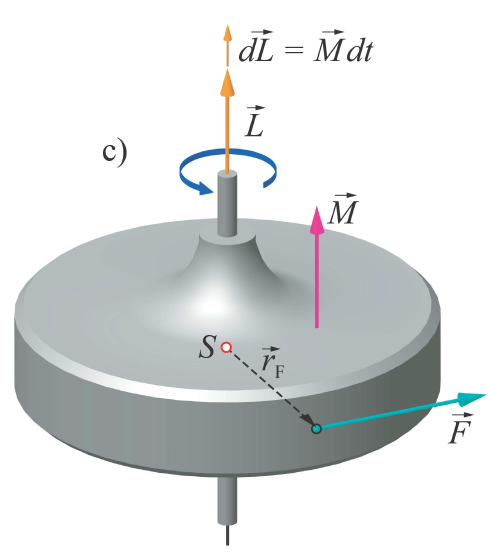
\includegraphics[width=\linewidth]{Bilder/drehimpuls} \\
			\\
		\end{minipage}
		\hfill
		\begin{minipage}{0.56\linewidth}
			$$ \boxed{ \vec{L} = \int d \vec{L} = \int \vec{r} \times \vec{v} \cdot dm = \vec{r} \times \vec{p} }$$ \\
		\end{minipage}

		\begin{tabular}{c l c}
			$\vec{L}$ & Drehimpuls & $[\vec{L}] = \mathrm{\frac{kg \, m^2}{s}}$ \\
			$\vec{r}$ & Abstand Massepunkt zu Rot-Achse & $[\vec{r}] = \mathrm{m}$ \\
			$\vec{v}$ & Rotationsgeschwindigkeit & $[\vec{v}] = \mathrm{\frac{m}{s}}$ \\
			$dm$ & kleines Masse-Stück & $[dm] = \mathrm{kg}$ \\
			$\vec{p}$ & Impuls & $[\vec{p}] = \mathrm{\frac{kg \, m}{s}}$ \\
		\end{tabular}

		\subsubsection{Energie beim Runterrollen}

			$$ \boxed{E_{pot} = E_{kin} + E_{rot} , \quad \quad m \cdot g \cdot h = \frac{1}{2}m \cdot v^2 + \frac{1}{2}J \cdot \omega^2} $$

		\subsubsection{Drehmoment $\vec{M}$ vs. Drehimpuls $\vec{L}$}
			$$ \boxed{ \vec{M} = \vec{r} \times \vec{F} = \frac{d}{dt} (\vec{r} \times \vec{p}) =  \frac{d}{dt} \vec{L} = \dot{\vec{L}} }$$ \\
			
			\textbf{In einem abgschlossenen System ($\vec{M} = 0$) bleibt der \\
			Gesamtdrehimpuls erhalten} \\
			$\Rightarrow \vec{L} = \text{const}$ \\
			\\
			\boxed{
				\begin{tabular}{ll}
					Impulserhaltung: &  $L  \overset{!}{=} L'$ \\
					& $J_1 \cdot \omega + J_2 \cdot \omega \overset{!}{=} J_1 \cdot \omega_1' + J_2 \cdot \omega_2'$ \\
					\\
					Energiesatz: & $E_{rot} \overset{!}{=} E_{rot}' + Q$ \\
					& $\frac{1}{2} J_1 \cdot \omega_1^2 + \frac{1}{2} J_2 \cdot \omega_2^2 \overset{!}{=} \frac{1}{2} J_1 \cdot \omega_1'^2 + \frac{1}{2} J_2 \cdot \omega_2'^2 + Q $ \\
				\end{tabular}
			}
			\\
			\\
			\begin{tabular}{c l c}
				$\vec{M}$ & Drehmoment & $[\vec{M}] = \mathrm{Nm}$ \\
				$\vec{r}$ & Abstand Massepunkt zu Rot-Achse & $[\vec{r}] = \mathrm{m}$ \\
				$\vec{F}$ & Kraft, welche Drehmoment bewirkt & $[\vec{F}] = \mathrm{N}$ \\
				$\vec{p}$ & Impuls & $[\vec{p}] = \mathrm{\frac{kg \, m}{s}}$ \\
				$\vec{L}$ & Drehimpuls & $[\vec{L}] = \mathrm{\frac{kg \, m^2}{s}}$ \\
				$J$  & Massenträgheitsmoment & $[J] = \mathrm{kg \, m^2}$ \\
				$\omega$ & Winkelgeschwindigkeit & $[\omega] = \mathrm{\frac{1}{s}}$ \\
				$Q$ & Deformationsarbeit & $[Q] = \mathrm{J}$ \\
			\end{tabular}

		\subsubsection{Drehimpuls $\vec{L}$ vs. Winkelgeschwindigkeit $\omega$}

		$$ \boxed{ L = \int dL = \int r^2 \, \omega \, dm = \omega \int r^2 \, dm = J \, \omega }$$ \\
		
			\begin{tabular}{c l c}
				$L$ & Drehimpuls & $[L] = \mathrm{\frac{kg \, m^2}{s}}$ \\
				$r$ & Abstand Massepunkt zu Rot-Achse & $[r] = \mathrm{m}$ \\
				$dm$ & kleines Masse-Stück & $[dm] = \mathrm{kg}$ \\
				$\omega$ & Winkelgeschwindigkeit & $[\omega] = \mathrm{\frac{rad}{s}}$ \\
				$J$ & (Massen-) Trägheitsmoment (hier Tensor) & $[J] = \mathrm{kg \, m^2}$ \\
			\end{tabular}

	\subsection{Rotation vs. Translation}
	
		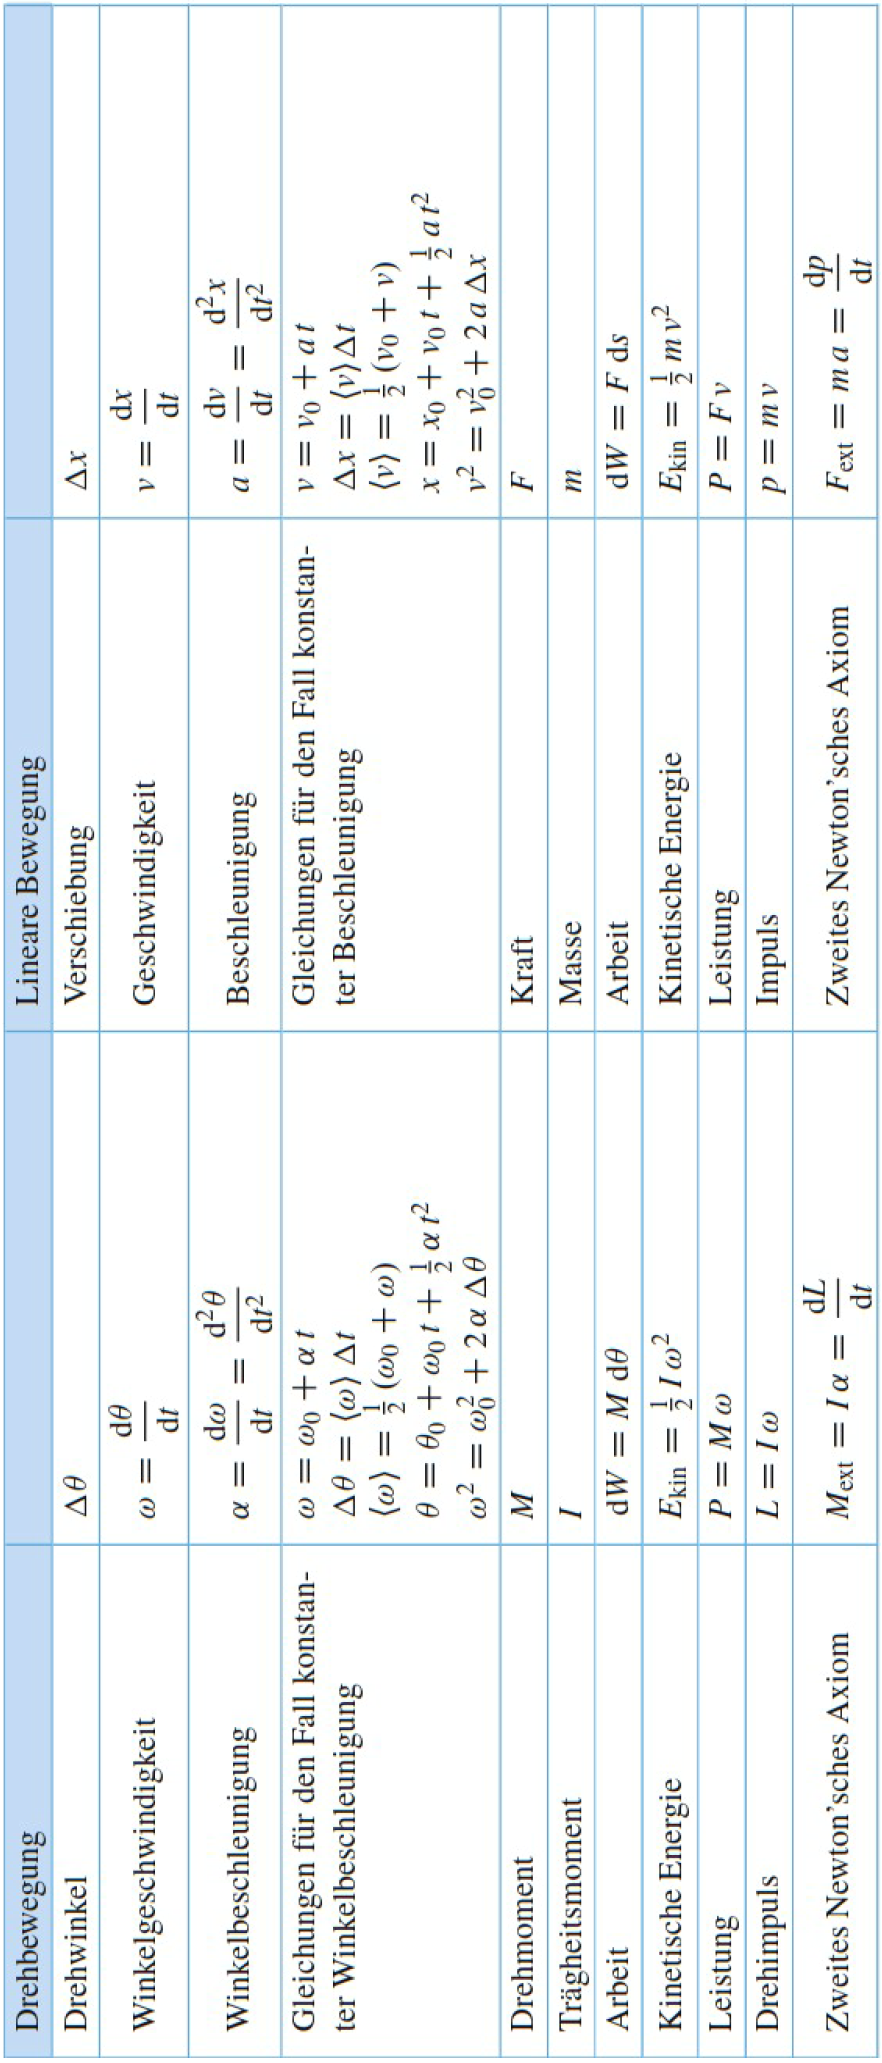
\includegraphics[width=0.85\linewidth]{Bilder/rotation_translation}
		
		%Code geputzt, Inhalt noch pendent

		\section{Vektorrechnung}
		
	\subsection{Betrag eines Vektors}
	$$ \vert \vec{A} \vert =  \sqrt{A_x^2 + A_y^2 + A_z^2}$$
		
		
	\subsection{Gleichheit zweier Vektoren}
	Zwei Vektoren sind gleich, wenn alle Komponenten identisch sind: \\
	\\
	\begin{tabular}{ll}
	$\bullet$ & $A_x = B_x$\\
	$\bullet$ & $A_y = B_y$\\
	$\bullet$ & $A_z = B_z$\\
	\end{tabular}		
		

		
		
	\subsection{Negative eines Vektors}
	\begin{minipage}{0.6\linewidth}
	\begin{tikzpicture}
		[
		x=1cm, y=1cm, scale=0.65, font=\footnotesize, >=latex 
		%Voreinstellung für Pfeilspitzen
		]
		
		%Raster links im Hintergrund
		\draw[step=1, gray, very thin] (0,0) grid (3.25,2.25);
		
		%Länge x Achse
		\draw [-latex] (0,0) -- ++(3.5,0) node[below] {$x$};
		
		%Länge y Achse
		\draw [-latex] (0,0) -- ++(0,2.5) node[left] {$y$};	
		
		%Vektor a
		\draw[-latex, red, very thick] (0.5,0.5) -- ++(2,1) node [midway, above] {$\vec{a}$} node (a) {}; 
		
		\draw[dashed] (a.center) ++ (-3,0) node (c) {};
		
		%Raster links im Hintergrund
		\draw[step=1, gray, very thin] (4,0) grid (7.25,2.25);
		
		%Länge x Achse
		\draw [-latex] (4,0) -- ++(3.5,0) node[below] {$x$};
		
		%Länge y Achse
		\draw [-latex] (4,0) -- ++(0,2.5) node[left] {$y$};	
		
		%Vektor a
		\draw[-latex, red, very thick] (6.5,1.5) -- ++(-2,-1) node [midway, above] {$\vec{b}$} node (a) {}; 
		
	\end{tikzpicture}
	\end{minipage}
	\hfill
	\begin{minipage}{0.3\linewidth}
	$b_x = - a_x$ \\
	\\
	$b_y = - a_y$ \\
	\\
	$b_z = - a_z$ \\
	\end{minipage}	
		
		
	
	\subsection{Addition zweier Vektoren}
	
	\begin{minipage}{0.6\linewidth}
	\begin{tikzpicture}
		[
		x=1cm, y=1cm, scale=0.7, font=\footnotesize, >=latex 
		%Voreinstellung für Pfeilspitzen
		]
		
		%Raster im Hintergrund
		\draw[step=1, gray, very thin] (0,0) grid (5.5,3.5);
		
		%Zahlen auf x-Achse
		\foreach \x in {0,1,2,3,4,5}
		\draw[shift={(\x,0)},color=black] (0pt,2pt) -- (0pt,-2pt) node[below]
		{\footnotesize $\x$};
		%Länge x Achse
		\draw [-latex] (0,0) -- ++(5.5,0) node[below] {$x$};
		%Länge y Achse
		\draw [-latex] (0,0) -- ++(0,3.5) node[left] {$y$};
		
		%Zahlen auf y-Achse
		%\foreach \y in {0,...,1}
		\foreach \y in {0,1,2,3}
		\draw[shift={(0,\y)},color=black] (2pt,0pt) -- (-2pt,0pt) node[left]
		{\footnotesize $\y$};		
		
		%Vektor a
		\draw[-latex, thick] (0,0) -- (2,3) node [midway, above] {$\vec{a}$} node (a) {}; 
		%Vektor b
		\draw[-latex, thick] (0,0) -- (3,0) node [midway, above] {$\vec{b}$} node (b) {}; 
		\draw[dashed] (a.center) -- ++ (3,0) node (c) {};
		\draw[dashed] (b.center) -- ++ (2,3);
		\draw[very thick, red, -latex] (0,0) -- (c.center) node [midway, above] {$\vec{c}$};
	\end{tikzpicture}
	\end{minipage}
	\hfill
	\begin{minipage}{0.3\linewidth}
	$c_x = a_x + b_x$ \\
	\\
	$c_y = a_y + b_y$ \\
	\\
	$c_z = a_z + b_z$ \\
	\end{minipage}
	
	
		
		
		
	\subsection{Subtraktion zweier Vektoren}
	
	\begin{minipage}{0.6\linewidth}
	\begin{tikzpicture}
		[
		x=1cm, y=1cm, scale=0.8, font=\footnotesize, >=latex 
		%Voreinstellung für Pfeilspitzen
		]
		
		%Raster im Hintergrund
		\draw[step=1, gray, very thin] (-0.5,-0.5) grid (6.5,2.5);
		
		%Zahlen auf x-Achse
		%\foreach \x in {0,1,2,3}
		%\draw[shift={(\x,0)},color=black] (0pt,2pt) -- (0pt,-2pt) node[below]
		%{\footnotesize $\x$};
		
		%Länge x Achse
		\draw [-latex] (0,0) -- (6.5,0) node[below] {$x$};
		
		%Länge y Achse
		\draw [-latex] (0,0) -- ++(0,2.5) node[left] {$y$};	
		
		%Vektor a
		\draw[-latex, very thick] (0,0) -- (3,2) node [midway, above] {$\vec{a}$} node (a) {}; 
		
		%Vektor b
		\draw[-latex, dashed, very thick] (3,2) -- ++(3,0) node [midway, above] {$\vec{b}$} node (b) {};
		\draw[-latex, very thick, blue] (3,2) -- ++(-3,0) node [midway, above] {$-\vec{b}$} node (-b) {}; 
		\draw[dashed] (a.center) ++ (-3,0) node (c) {};
		
		%\draw[dashed] (-b.center) -- ++ (2,3);
		%\draw[dashed] (b.center) -- ++ (-1,3);
		\draw[very thick, red, -latex] (0,0) -- (c.center) node [midway, left] {$\vec{c}$};
		
		%Zahlen auf y-Achse 
		%\foreach \y in {0,...,1}
		%\foreach \y in {1,2,3}
		%\draw[shift={(0,\y)},color=black] (2pt,0pt) -- (-2pt,0pt) node[left]
		%{\footnotesize $\y$};	
	\end{tikzpicture}
	\end{minipage}
	\hfill
	\begin{minipage}{0.3\linewidth}
	$c_x = a_x - b_x$ \\
	\\
	$c_y = a_y - b_y$ \\
	\\
	$c_z = a_z - b_z$ \\
	\end{minipage}	
		
		
	\subsection{Multiplikation eines Vektros mit einem Skalar}
	\begin{minipage}{0.68\linewidth}
	$$\vec{b} = s \, \vec{a} \quad \vert \vec{B} \vert = \vert s \vert \cdot \vert \vec{a} \vert$$ \\
	\end{minipage}
	\hfill
	\begin{minipage}{0.3\linewidth}
	$b_x = s \cdot a_x$ \\
	\\
	$b_y = s \cdot a_y$ \\
	\\
	$b_z = s \cdot a_y$ \\
	\end{minipage}	
	
		
		
		
		
	\subsection{Skalarprodukt}
	$$\vec{c} = \vec{a} \bullet \vec{b} = \vert \vec{a} \vert \cdot \vert \vec{b} \, \vert  \, \cos(\varphi)$$ 
		
		
		
		
		
	\subsection{Kreuzprodukt (nur in 3D)}
	 $$\vec{a} \times \vec{b} = \begin{pmatrix} a_2 b_3 - a_3 b_2 \\ -(a_1 b_3 - a_3 b_1) \\ a_1 b_2 - a_2 b_1 \end{pmatrix}$$ 
		
				


		\section{Statistik}
	\subsection{Arithmetisches Mittel $\overline{x}_{arith}$}
		
	$\overline{x}_{arith} := \frac{1}{N} \sum \limits_{i = 1}^N  x_i$
	
		
		
	\subsection{Geometrisches Mittel $\overline{x}_{geom}$}
	\textbf{Nur für positive Zahlenreihen $x_i$ definiert!} \\
	\\		
	$\overline{x}_{geom} := \sqrt[N]{\prod \limits_{i = 1}^N  x_i }$ \qquad \qquad $\Rightarrow \overline{x}_{geom} \leq \overline{x}_{arith}$
		
		
		
	\subsection{Quadratisches Mittel QMW (RMS)}
	\textbf{Wechselstromtechnik; Effektivwert} \\
	\\
	$QMW := \sqrt{ \frac{1}{N} \sum \limits_{i = 1}^N  x_i^2 }$
		
		
	\subsection{Harmonisches Mittel $\overline{x}_{harm}$}		
	
	$\overline{x}_{harm} := \frac{N}{ \sum \limits_{i = 1}^N   \frac{1}{x_i} } $ \\
	\\
	Kann sinnvoll eingesetzt werden, wenn man für die $i-te$ Teilstrecke $s_i$ eine Zeit $t_i$ benötigt (also eine Durchschnittsgeschwindigkeit von $v_i = \frac{s_i}{t_i}$ und eine Durchschnittsgeschwindigkeit über $N$ Teilstrecken ermitteln will: \\
	\\
	$\overline{v}_{harm} = \frac{\sum \limits_{i = 1}^N  s_i }{\sum \limits_{i = 1}^N  t_i} = \frac{\sum \limits_{i = 1}^N  s_i }{\sum \limits_{i = 1}^N \frac{s_i}{v_i} }  $ \qquad gewichtetes harm. Mittel
		
		
		
	\subsection{Standardabweichung $\sigma$}	
		
	\begin{tabular}{ll}
	Varianz: & $\sigma^2 := \frac{1}{N} \sum \limits_{i = 1}^N (x_i - \overline{x}_{arith} )^2 $ \\
	\\
	Standardabweichung: &  $\sigma := \sqrt{ \frac{1}{N} \sum \limits_{i = 1}^N (x_i - \overline{x}_{arith} )^2 }$ \\
	\end{tabular}
		
		
		
	\subsection{Standardabweichung des Mittelwerts}	
	\textbf{Gilt nur, wenn eine Normalverteilung vorliegt!} \\
	Beschreibt nur statistische Fehler \\
	\\
	$\sigma(\overline{x}_{arith}) = \frac{\sigma}{\sqrt{N}} $
		
		

		\section{Mathematik-Hilfe}
		
	\subsection{Trigonometrie}
	\begin{tabular}{| c | c | c |}
	\hline
	Sinus & Cosinus & Tangens \\ 
	\hline 
	\rule{0pt}{10pt} $\frac{GK}{H}$ & $\frac{AK}{H}$ & $\frac{AK}{GK}$ \\ 
	\hline
	\end{tabular} 
		
		
		
	\subsection{Schwerpunkt}
	Die Koordinaten des Schwerpunkts müssen komponentenweise berechnet werden: \\
	\\
	$x_s = \frac{\sum  x_i \cdot m_i}{M}$ \qquad	$y_s = \frac{\sum  y_i \cdot m_i}{M}$ \qquad $z_s = \frac{\sum  z_i \cdot m_i}{M}$ \\
	\\
	\begin{tabular}{ll}
	$x_s \; , y_s \; , z_s$ & Koordinaten des Schwerpunkts \\
	$x_i \; , y_i \; , z_i$ & Koordinaten von kleinen Massepunkten \\
	$m_i$ & Kleine Massepunkte an entsprechenden Koordinaten \\
	$M$ & Gesamtmasse des Körpers
	\end{tabular}
	
	\subsection{Polarkoordinaten (Kreisbewegung)}

	
	\begin{tabular}{ll}
	polar $\rightarrow$ kartesisch & $\vec{P} =  \begin{pmatrix} x \\ y \end{pmatrix} =  \begin{pmatrix} r \cdot \cos(\phi)  \\ r \cdot \sin(\phi)  \end{pmatrix}$ \\
	\\
	kartesisch $\rightarrow$ polar & $\vec{P} =  \begin{pmatrix} r \\ \phi \end{pmatrix} =  \begin{pmatrix} \sqrt{x^2 + y^2}  \\ \tan \big( \frac{x}{y} \big)   \end{pmatrix}$\\
	\end{tabular}
	
	
	
	\subsection{Ableitungsregeln S .445-448}
			
			\subsubsection{Elementare Regeln}
			\begin{tabular}{lll}
			Potenzen: & $f(x) = x^3$ & $f'(x) = 3 \, x^2$ \\
			& $f(x) = x^\alpha$ & $f'(x) = \alpha \cdot x^{\alpha - 1}$ \\
			\\
			Linearität: & $f(x) = c \cdot x^2$ & $f'(x) = c \cdot 2 \, x $ \\
			\\
			Summe: & $(u(x) + v(x) - w(x))' $ & = $u'(x) + v'(x) - w'(x)$ \\
			\\
			Konstanten: & $c = const$ $\rightarrow$ $c' = 0$ \\
			\end{tabular}
			
			
			\subsubsection{Produktregel}
			$(f(x) \cdot g(x))' = f'(x) \cdot g(x) + f(x) \cdot g'(x)$ 
			
			\subsubsection{Quotientenregel}
			$\left( \frac{u(x)}{v(x)} \right) ' = \frac{u'(x) \cdot v(x) - u(x) \cdot v'(x)}{v(x) ^2}$ \quad $\rightarrow$ als Produkt schreiben \\
			\\
			$u(x) \cdot \left( \frac{1)}{v(x)} \right) ' =  u'(x) \cdot \frac{1}{v(x)} + u(x) \cdot \frac{- v'(x)}{v(x)^2}$
			
			\subsubsection{Kettenregel}
			$g(f(x))' =  f'(x) \cdot g'(x)$ \\
			
			\subsubsection{Umkehrfunktion}
			$(f^{-1}(y_0))' = \frac{1}{f'(x_0)} =  \frac{1}{f'(f^{-1}(y_0))}$ \\
			

			
			\subsection{Allgemeine Logarithmus-Ableitung}
			$(\log_b(x))' = \left( \frac{\ln(x)}{\ln(b)} \right)' = \frac{1}{\ln(b)} \cdot (\ln(x))' = \frac{1}{\ln(b)} \cdot \frac{1}{x} $
			
			
			
			
			\subsection{Integrationsregeln S. 494-496}
		Linearität: $\int \limits_{a}^{b} \alpha \, f(x) \, dx = \alpha \int \limits_{a}^{b} f(x) \, dx$ 
		
		
		\subsubsection{Rechenregeln mit Integralen S. 508-510}
		\begin{tabular}{ll}
		Zerlegung: & $\int \limits_{a}^{b} f_1(x) \, dx + f_2(x) \, dx = \int \limits_{a}^{b} f_1(x) \, dx + \int \limits_{a}^{b} f_2(x) \, dx$ \\
		\\		
		& $\int \limits_{a}^{c} f(x) \, dx = \int \limits_{a}^{b} f(x) \, dx + \int \limits_{b}^{c} f(x) \, dx$ \\
		\\
		Grenzen tauschen: & $ \int \limits_{a}^{b} f(x) \, dx = -  \int \limits_{b}^{a} f(x) \, dx $ \\
		\\
		Gleiche Grenzen: &  $\int \limits_{a}^{a} f(x) \, dx = 0$ \\
		\end{tabular}
		
		
		\subsection{Wichtige Integrale S. 495}
		\begin{tabular}{ll}
		$\int \limits_{a}^{b} x^2  \, dx = \frac{b^3}{3} - \frac{a^3}{3}$ & $\int \limits_{a}^{b} x \, dx = \frac{b^2}{2} - \frac{a^2}{2}$ \\
		\\
		$\int \limits_{a}^{b} 1 \, dx = b - a $ (Rechteck)& \\
		\end{tabular}
			
	
	
		
	\end{multicols*}	
\end{document}